\documentclass[11pt]{article}
\usepackage[T1]{fontenc}
\usepackage[utf8]{inputenc}
\usepackage{lmodern}
\usepackage[a4paper,margin=2.6cm]{geometry}
\usepackage{amsmath,amssymb,amsthm}
\usepackage{booktabs}
\usepackage{graphicx}
\usepackage[round,authoryear]{natbib}
\usepackage[hidelinks]{hyperref}
\usepackage{xcolor}
\usepackage{microtype}
\pdfstringdefDisableCommands{\def\xi{xi}\def\rho{rho}}

\newtheorem{theorem}{Theorem}
\newtheorem{proposition}{Proposition}
\newtheorem{lemma}{Lemma}
\newtheorem{corollary}{Corollary}
\theoremstyle{definition}
\newtheorem{assumption}{Assumption}
\newtheorem{definition}{Definition}
\theoremstyle{remark}
\newtheorem{remark}{Remark}

\numberwithin{equation}{section}

\newcommand{\R}{\mathbb{R}}
\newcommand{\Prob}{\mathbb{P}}
\newcommand{\E}{\mathbb{E}}
\newcommand{\dto}{\rightsquigarrow}
\newcommand{\Mesh}{\mathcal{M}}

% generated by scripts/build_preprint_assets.py
\newcommand{\DoneA}{14}
\newcommand{\DoneB}{16}
\newcommand{\Dthree}{15}
\newcommand{\Dtwo}{12}
\newcommand{\GammaMinR}{0.945}
\newcommand{\GammaOutA}{0.924}
\newcommand{\GammaOutB}{0.739}
\newcommand{\GammaOutC}{0.168}
\newcommand{\GammaOutD}{0.000}
\newcommand{\GammaZeroMin}{0.947}
\newcommand{\GminOne}{0.944}
\newcommand{\benchReps}{300}
\newcommand{\boundTwo}{0.900}
\newcommand{\cOneEnd}{2.203}
\newcommand{\cTwoEnd}{2.201}
\newcommand{\cgpSimIn}{0.76--0.94}
\newcommand{\cgpSimInN}{14}
\newcommand{\danishClip}{$k=19$: upper end 2.60}
\newcommand{\danishGH}{84}
\newcommand{\danishInter}{[0.523, 0.843]}
\newcommand{\danishKgh}{79}
\newcommand{\danishKs}{19, 39, 79, 158, 317}
\newcommand{\danishKsam}{317}
\newcommand{\danishN}{2167}
\newcommand{\danishSamsee}{959}
\newcommand{\deltaRatioIn}{0.62}
\newcommand{\deltaRatioOut}{0.97--0.98}
\newcommand{\diffAbsMax}{0.046}
\newcommand{\diffIn}{\ensuremath{-0.023} to \ensuremath{+0.046}}
\newcommand{\finDn}{0.039}
\newcommand{\finOneFactor}{5}
\newcommand{\finUp}{0.060}
\newcommand{\foLepskiMin}{0.03}
\newcommand{\foLepskiN}{12}
\newcommand{\foLepskiRange}{0.027--0.793}
\newcommand{\gpSimIn}{0.713--0.943}
\newcommand{\kappaWorst}{0.902}
\newcommand{\lamBenchMax}{13.9}
\newcommand{\lamMax}{48}
\newcommand{\limitKs}{64, 128, 256, 512, 1024}
\newcommand{\meshInsensitive}{identical}
\newcommand{\nCellsIn}{16}
\newcommand{\nEndpointDraws}{1{,}000{,}000}
\newcommand{\nRhoEval}{61}
\newcommand{\obsIn}{0.920--0.997}
\newcommand{\obsOut}{0.147--0.790}
\newcommand{\piTwoMax}{0.0501}
\newcommand{\posthocAvailable}{1}
\newcommand{\predIn}{0.943--0.954}
\newcommand{\predOut}{0.877--0.900}
\newcommand{\qMax}{0.00007}
\newcommand{\rhoFrechetSwitch}{\ensuremath{-2.25}}
\newcommand{\rhoNineBurrA}{\ensuremath{-0.44}}
\newcommand{\rhoNineBurrB}{\ensuremath{-0.59}}
\newcommand{\rhoNineBurrC}{\ensuremath{-1.00}}
\newcommand{\rhoNineBurrCsmall}{\ensuremath{-0.85} (interquartile range \ensuremath{-1.23} to \ensuremath{-0.65})}
\newcommand{\rhoNineFrechet}{\ensuremath{-1.05}}
\newcommand{\rhoNineNineNineBurrA}{\ensuremath{-0.73}}
\newcommand{\rhoNineNineNineBurrB}{\ensuremath{-0.76}}
\newcommand{\rhoNineNineNineBurrC}{\ensuremath{-0.84}}
\newcommand{\seBench}{0.017}
\newcommand{\seLimit}{0.002}
\newcommand{\simsLimit}{20000}
\newcommand{\swGHIn}{0.81--0.98}
\newcommand{\swSnoopBurr}{0.13--0.40}
\newcommand{\swSnoopGood}{0.96--1.00}
\newcommand{\swSnoopOut}{0.00}
\newcommand{\swSnoopWidthRatio}{0.64--0.90}
\newcommand{\swTopBurr}{0.00--0.06}
\newcommand{\swTopGoodMin}{0.98}
\newcommand{\swTopIn}{0.00--1.00}
\newcommand{\swWidthRatio}{0.57--0.82}
\newcommand{\unionPostMinIn}{0.947}
\newcommand{\unionSimIn}{0.920--0.997}
\newcommand{\unionSimOut}{0.147--0.790}
\newcommand{\unionVsPluginWidth}{1.2--2.1}
\newcommand{\upperTwo}{0.950}
\newcommand{\widthOneSided}{0.1}
\newcommand{\widthRatioMax}{7.8}
\newcommand{\widthRatioZero}{2.0}


\title{Selection-valid inference for the tail index under second-order bias\\ without estimating the second-order parameter}
\author{Ziyi Zhou\thanks{Independent Researcher, Montr\'eal, Canada.}}
\date{Preprint, \today}

\begin{document}
\maketitle

\begin{abstract}
The tail index $\xi$ of a heavy-tailed distribution is estimated from the $k$ largest observations, and $k$ is chosen after looking at the data, yet the interval reported for $\xi$ is the one computed at the selected $k$ as if $k$ had been fixed; under second-order bias its coverage can be close to zero. We study intervals that keep frequentist coverage after any data-driven choice of $k$ from a fixed grid, when the bias $\sqrt{k}\,\delta\{U(n/k)\}$ has a possibly non-zero limit, and without estimating the second-order parameter $\rho$. The intervals are convex hulls, over a range of working values of $\rho$, of simultaneous credible bands from an extended-Pareto posterior. Taking unions over a nuisance range is a classical device; our contribution is its analysis in this problem. We prove a Bernstein--von Mises theorem for the posterior at a misspecified working value, with an explicit asymptotic bias, and derive the limiting coverage and width of the hull: the coverage is bounded below uniformly over the range of $\rho$ and the bias limit, and the width is of order $k^{-1/2}$. A pre-registered simulation study and an application to Danish fire insurance losses illustrate the method.
\end{abstract}

\noindent\textit{Keywords:} extreme value index; threshold selection; post-selection inference; second-order regular variation; Bernstein--von Mises theorem; extended Pareto distribution.

\section{Introduction}\label{sec:intro}

Let $X_1,\dots,X_n$ be independent with a distribution function $F$ in the Fr\'echet domain of attraction, $1-F(x)=x^{-1/\xi}\ell(x)$ with $\xi>0$ and $\ell$ slowly varying. Inference on $\xi$, and on extreme quantiles that depend on it, uses the $k$ largest observations. The choice of $k$ trades bias, which grows with $k$, against variance, which shrinks with it. In practice $k$ is chosen from the data: from a Hill plot, by an automatic rule \citep{dreeskaufmann1998,guillouhall2001,schneider2021}, or by a stability criterion. The interval then reported for $\xi$ is the one computed at the selected $\hat k$ as if $\hat k$ had been fixed in advance. Nothing guarantees its coverage. In the simulation of Section~\ref{sec:sim}, the nominal 90\% first-order interval at a stability-selected $\hat k$ covered $\xi$ in as few as \foLepskiMin{} of samples, and below $0.80$ in \foLepskiN{} of \nCellsIn{} settings.

Two obstacles meet here. First, a reported interval should remain valid after $k$ is selected, which is a post-selection problem \citep{berk2013}; a supremum over the tuning parameter is the standard remedy in nonparametric regression \citep{armstrongkolesar2018snoop}. Second, selection rules tend to choose $k$ where the second-order bias is not negligible, so the interval at each $k$ must be valid when $\sqrt{k}A(n/k)$ does not vanish. The standard way to remove that bias requires the second-order parameter $\rho$, either through an external estimate \citep{gomesmartins2002,cgp2005} or through the extended Pareto model \citep{bjs2009}; consistent estimators of $\rho$ exist \citep{fagh2003}, but at the auxiliary threshold used in practice they converge very slowly \citep[\S2]{cgp2005}, and in our experience estimates at practical sample sizes can be far from $\rho$ (Section~\ref{sec:rhohat}). Alternatively, \citet{sasakiwang2024} construct intervals that are uniformly valid over a local class by adding a worst-case bias bound, which requires the user to supply bounds $(A,\rho)$ on the second-order deviation; their snooping interval, an intersection over a range of thresholds, is uniformly valid over that range and therefore also after a data-driven choice of threshold within it. \citet{carpentierkim2014} construct honest adaptive intervals over a second-order class with a known range for the second-order exponent and a separation condition, without tight constants. Intervals for the Hill estimator at a fixed $k$ are compared by \citet{chengpeng2001} and \citet{haeuslersegers2007}, and fixed-$k$ asymptotics avoid second-order assumptions altogether at the price of using few order statistics \citep{mullerwang2017}. Bayesian tail posteriors have Bernstein--von Mises theorems; for $\sqrt{k}A(n/k)\to\lambda\neq0$ their centre is biased, and their coverage results are for $\lambda=0$ \citep{dombry2023}.

This paper asks what can be guaranteed without an estimate of $\rho$ and without a user-supplied bias bound, assuming only that $\rho$ lies in a stated range. The price is that our guarantees are pointwise in the distribution; by the lower bound of \citet[Theorem~1]{sasakiwang2024}, a bias bound cannot be avoided for intervals that are uniformly valid over a local class. We use simultaneous bands along a fixed grid of $k$, which give post-selection validity by an inclusion that holds in every finite sample; we centre them at extended-Pareto (EPD) posteriors, which remove the leading bias at the correct $\rho$; and we take the convex hull of the bands computed at a finite mesh of working values $\rho'$. The last step is the classical device of taking a union, or supremum, over a nuisance range (cf.\ \citealp{bergerboos1994}, who restrict it to a confidence set for the nuisance parameter, and \citealp{silvapulle1996}). Its textbook justification covers only the case where the true $\rho$ is in the union. Our analysis shows what happens for the finite mesh actually computed.

\paragraph{Contributions.}
\begin{enumerate}
\item \emph{The posterior at a wrong working value} (Theorem~\ref{thm:bvm}, Lemma~\ref{lem:beta}). Under a local second-order model, the EPD posterior computed at any fixed $\rho'<0$ satisfies a Bernstein--von Mises theorem whose centre has asymptotic bias $\lambda\beta(\rho,\rho')$, with $\beta$ in closed form and $\operatorname{sign}\beta(\rho,\rho')=\operatorname{sign}(\rho'-\rho)$, jointly along a grid of thresholds and a mesh of working values. The proof uses local asymptotic normality along the second-order direction and Le Cam's third lemma; the limiting Gaussian law has a covariance in closed form (Appendix~\ref{app:cov}).
\item \emph{Exact asymptotics of the finite-mesh union band} (Theorem~\ref{thm:union}). The limiting simultaneous coverage $\Gamma_\Mesh(\rho,\lambda)$ and width are explicit Gaussian functionals. As a function of the bias limit the coverage tends to one as $|\lambda|\to\infty$ when $\rho$ lies strictly between mesh points, and to zero when $\rho$ lies outside the mesh range. The width keeps the rate $k^{-1/2}$ for each fixed $\lambda$, with a constant that grows linearly in $|\lambda|$.
\item \emph{A coverage bound on the whole range} (Theorem~\ref{thm:uniform}, Corollary~\ref{cor:uniform}, Propositions~\ref{prop:tight} and~\ref{prop:cex}). For all $\rho\in R$ and all $\lambda$, $\Gamma_\Mesh\ge1-\varphi_\Mesh$, with $\varphi_\Mesh$ determined by the two endpoint bands alone. With one-sided calibration of those two bands the band has limiting coverage at least $1-\alpha$ on $R$ uniformly in $\lambda$; with the implemented two-sided calibration the guarantee is $1-\alpha-\tfrac12(q_1+q_L)$, and an example shows that bracketing alone cannot close this gap. The infimum lies between $1-\varphi_\Mesh$ and $1-\max(\pi_1,\pi_L)$, and in the abstract sign-constrained class the bound $1-\varphi_\Mesh$ is attained.
\item \emph{Evidence} (Section~\ref{sec:sim}). In a pre-registered simulation the band kept coverage after four selection rules in all \nCellsIn{} settings within the stated range, and in a post hoc comparison a finite-$k$ approximation of $\Gamma_\Mesh$ was within \diffAbsMax{} of its simultaneous coverage there. The theory does not predict a failure for slow second-order decay, which we report.
\end{enumerate}

\paragraph{What is not new.} The union over a nuisance range \citep{bergerboos1994,silvapulle1996}; post-selection validity through simultaneity \citep{berk2013,armstrongkolesar2018snoop}, including for the tail index with an intersection over thresholds \citep[eq.~15]{sasakiwang2024}; process limits of tail estimators along $k$ \citep{drees1998,ddhr2000}; worst-case-bias intervals for the tail index \citep{sasakiwang2024}, in the spirit of \citet{armstrongkolesar2018,armstrongkolesar2020}; and the use of the joint structure of estimators across thresholds for threshold selection \citep{wadsworth2016,northropcoleman2014,murphy2025}. The frequentist twin of our band (the EPD estimator of \citealp{bjs2009} with the same calibration) has the same limiting coverage and width; the Bayesian construction is a convenient way to compute it, and its frequentist guarantee is the subject of this paper.

\paragraph{Credible level versus coverage.} Each band is a central posterior credible interval at an inflated level $1-\alpha^*$, chosen so that the bands hold simultaneously with frequentist probability $1-\alpha$. All guarantees below are statements about frequentist coverage under repeated sampling from $F$. We make no claim about the posterior probability of the hull.

\section{Framework and assumptions}\label{sec:framework}

Write $\bar F=1-F$ and $U(t)=F^{\leftarrow}(1-1/t)$. Let $X_{1,n}\le\dots\le X_{n,n}$ be the order statistics.

\begin{assumption}[second-order tail]\label{ass:A1}
There are $\xi>0$, $\rho<0$, $C>0$ and $x_0$ such that $\bar F(x)=Cx^{-1/\xi}\{1+\xi^{-1}\delta(x)\}$ for $x\ge x_0$, where $\delta$ is eventually of constant sign and $|\delta|$ is regularly varying with index $\rho/\xi$.
\end{assumption}

This is the class of \citet[Def.~2.2]{bjs2009}, written with $\xi$ for their $\gamma$. It implies the usual second-order condition with auxiliary function $A(t)=\rho\,\delta\{U(t)\}\{1+o(1)\}$.

For $u>x_0$ let $q_u(y)=uf(uy)/\bar F(u)$, $y\ge1$, be the density of $X/u$ given $X>u$, and let $p(y)=\xi^{-1}y^{-1/\xi-1}$ be the Pareto density. Put
\begin{equation}\label{eq:h}
h_\rho(y)=\xi^{-1}\{(1-\rho)\,y^{\rho/\xi}-1\},\qquad y\ge1.
\end{equation}

\begin{assumption}[quadratic-mean second-order condition]\label{ass:A2}
$F$ has a density $f$ on $(x_0,\infty)$, and as $u\to\infty$,
$\int_1^\infty\{q_u^{1/2}-p^{1/2}-\tfrac12\delta(u)h_\rho\,p^{1/2}\}^2\,dy=o\{\delta(u)^2\}$.
\end{assumption}

Assumption~\ref{ass:A2} states that the relative excesses form a differentiable path through the Pareto model in the direction $h_\rho$. The direction is the one implied by Assumption~\ref{ass:A1}: differentiating $y^{-1/\xi}\{1+\xi^{-1}\delta(y^{\rho/\xi}-1)\}$ in $\delta$ gives $h_\rho$ (Lemma~\ref{lem:scores} in the Appendix). A sufficient condition is $q_u(y)/p(y)=1+\delta(u)h_\rho(y)+r_u(y)$ with $\sup_{y\ge1}|r_u(y)|y^{-\epsilon}=o\{\delta(u)\}$ for some $\epsilon<1/(4\xi)$ (Lemma~\ref{lem:suff}). We have not verified Assumption~\ref{ass:A2} separately for each distribution used in Section~\ref{sec:sim}.

\begin{assumption}[intermediate sequence and grid]\label{ass:A3}
$k=k_n\to\infty$, $k/n\to0$ and $\sqrt{k}\,\delta\{U(n/k)\}\to\lambda\in\R$. The grid is $k_j=\lfloor t_jk\rfloor$, $j=1,\dots,m$, with $0<t_1<\dots<t_m=1$ and $m$ fixed. Then $\sqrt{k_j}\,\delta\{U(n/k_j)\}\to\lambda_j:=\lambda\,t_j^{1/2-\rho}$.
\end{assumption}

All results are pointwise: $F$, hence $(\xi,\rho,\lambda)$, is fixed while $n\to\infty$. Assumption~\ref{ass:A3} with finite $\lambda$ is the regime in which the bias is of the same order as the standard deviation at every grid point; Remark~\ref{rem:R2} discusses $|\lambda|=\infty$.

\paragraph{Working model.} For $\rho'<0$, the extended Pareto distribution EPD$(\xi,\delta;\rho')$ on $(1,\infty)$ has survival function $\{y(1+\delta-\delta y^{\rho'/\xi})\}^{-1/\xi}$ \citep[Def.~2.1]{bjs2009}; at $\delta=0$ it is the Pareto distribution. At threshold $k_j$ the data are the relative excesses $Y^{(j)}_i=X_{n-i+1,n}/X_{n-k_j,n}$, $i\le k_j$.

\begin{assumption}[prior]\label{ass:P}
For each working value $\rho'$, the prior $\Pi_{\rho'}$ on $(\xi,\delta)$ has compact support contained in the set where the EPD density is valid and positive, and a density that is continuous and positive at $(\xi,0)$, which is an interior point of the support.
\end{assumption}

Write $\Pi_{j,\rho'}(\cdot\mid Y^{(j)})$ for the posterior of $\xi$ at threshold $k_j$ under the EPD$(\rho')$ likelihood. Define
\begin{equation}\label{eq:s}
s(\rho')=\frac{1-\rho'}{|\rho'|},\qquad
\beta(\rho,\rho')=\frac{\rho(1-\rho')(\rho'-\rho)}{\rho'(1-\rho)(1-\rho-\rho')}.
\end{equation}
Here $\xi s(\rho')$ is the asymptotic standard deviation of efficient estimators of $\xi$ in the EPD$(\rho')$ model at $\delta=0$.

\section{The posterior at a working value}\label{sec:bvm}

Let $E=\xi^{-1}\log Y$, $a_{\rho'}(E)=(1-\rho')e^{\rho'E}-1$ and
\[
\psi_{\rho'}(E)=\frac{(1-\rho')^2}{\rho'^2}(E-1)-\frac{(1-2\rho')(1-\rho')}{\rho'^3}\,a_{\rho'}(E),
\]
which is $\xi^{-1}$ times the efficient influence function for $\xi$ in the EPD$(\rho')$ model at $\delta=0$ (Lemma~\ref{lem:scores}). Define the centring
$\tilde\xi_j(\rho')=\xi\{1+k_j^{-1}\sum_{i\le k_j}\psi_{\rho'}(E^{(j)}_i)\}$ with $E^{(j)}_i=\xi^{-1}\log Y^{(j)}_i$, and let $\hat\xi_j(\rho')$ be the estimator of \citet{bjs2009} at $k_j$ with $\rho$ fixed at $\rho'$.

Let $G=(G_{jl})$ denote the centred Gaussian array that is the limit in distribution of $\{\sqrt{k_j}(\tilde\xi_j(\rho_l)-\xi)/\xi\}_{j,l}$ under exact Pareto tails ($\delta\equiv0$). By Lemma~\ref{lem:clt} in the Appendix its law depends only on $(t_j)$ and the working values, with
\begin{equation}\label{eq:cov}
\operatorname{cov}(G_{jl},G_{j'l'})=(t_j/t_{j'})^{1/2}\operatorname{cov}\{\psi_{\rho_l}(E),\psi_{\rho_{l'}}(E+\log(t_{j'}/t_j))\},\qquad t_j\le t_{j'},\ E\sim\mathrm{Exp}(1),
\end{equation}
and $\operatorname{var}(G_{jl})=s(\rho_l)^2$.

\begin{theorem}[posterior at fixed working values]\label{thm:bvm}
Assume \ref{ass:A1}--\ref{ass:A3} and \ref{ass:P}. Let $\rho_1,\dots,\rho_L<0$ be fixed. Then
\begin{enumerate}
\item[(i)] for every $j$ and $l$, $\sup_B\bigl|\Pi_{j,\rho_l}\{\sqrt{k_j}(\vartheta-\tilde\xi_j(\rho_l))\in B\mid Y^{(j)}\}-N\{0,\xi^2s(\rho_l)^2\}(B)\bigr|\to0$ in probability, where $\vartheta$ denotes the posterior variable;
\item[(ii)] jointly in $j\le m$, $l\le L$, $\sqrt{k_j}\{\tilde\xi_j(\rho_l)-\xi\}/\xi\dto G_{jl}+\mu_{jl}$ with $\mu_{jl}=(\lambda_j/\xi)\,\beta(\rho,\rho_l)$;
\item[(iii)] $\sqrt{k_j}\{\hat\xi_j(\rho_l)-\tilde\xi_j(\rho_l)\}\to0$ in probability.
\end{enumerate}
\end{theorem}

\begin{lemma}[bias at a working value]\label{lem:beta}
$\beta(\rho,\rho)=0$ and $\operatorname{sign}\beta(\rho,\rho')=\operatorname{sign}(\rho'-\rho)$. Relative to the Hill estimator, whose bias is $\lambda\rho/(1-\rho)$, the factor is $(1-\rho')(\rho'-\rho)/\{\rho'(1-\rho-\rho')\}$: negative for $\rho<\rho'<0$ (over-correction) and in $(0,1)$ for $\rho'<\rho$ (under-correction).
\end{lemma}

The proofs are in the Appendix. Theorem~\ref{thm:bvm} with $\rho_l=\rho$ gives the known-$\rho$ result: the posterior centre is asymptotically unbiased for every $\lambda$. The first-order (Pareto) posterior is the case $\delta\equiv0$; its centre is the Hill estimator, with bias $\lambda_j\rho/(1-\rho)$, and its bands under-cover (Proposition~\ref{prop:firstorder}).

\paragraph{Bands at one working value.} Let $c(\rho')$ be the $(1-\alpha)$-quantile of $\max_j|G_{jl}|/s(\rho')$ for $\rho_l=\rho'$, and $\alpha^*(\rho')=2\{1-\Phi(c(\rho'))\}$. The band at $\rho'$ is
\[
B_j(\rho')=\text{central }(1-\alpha^*(\rho'))\text{ posterior credible interval for }\xi\text{ under }\Pi_{j,\rho'},\qquad j=1,\dots,m.
\]

\begin{corollary}[known $\rho$]\label{cor:known}
Under the conditions of Theorem~\ref{thm:bvm}, $\Prob\{\xi\in B_j(\rho)\ \forall j\}\to1-\alpha$ for every $\lambda\in\R$.
\end{corollary}

\begin{proposition}[first-order bands]\label{prop:firstorder}
Let $B^{P}_j$ be the bands built in the same way from the Pareto posterior, calibrated under exact Pareto tails. If $\lambda\ne0$, $\lim\Prob\{\xi\in B^P_j\ \forall j\}<1-\alpha$, and the limit tends to $0$ as $|\lambda|\to\infty$.
\end{proposition}

\section{The finite-mesh union band}\label{sec:union}

Fix a mesh $\Mesh=\{\rho_1<\dots<\rho_L\}\subset(-\infty,0)$, write $R=[\rho_1,\rho_L]$, $s_l=s(\rho_l)$ and $c_l=c(\rho_l)$, and define the reported band as the hull
\begin{equation}\label{eq:U}
U_j=\Bigl[\min_{l}\inf B_j(\rho_l),\ \max_{l}\sup B_j(\rho_l)\Bigr],\qquad j=1,\dots,m.
\end{equation}
No estimate of $\rho$ enters $U_j$. Let
\[
\Gamma_\Mesh(\rho,\lambda)=\Prob\Bigl[\text{for all }j:\ \min_l\{G_{jl}+\mu_{jl}-c_ls_l\}\le0\le\max_l\{G_{jl}+\mu_{jl}+c_ls_l\}\Bigr].
\]

\begin{theorem}[finite-mesh union band]\label{thm:union}
Assume the conditions of Theorem~\ref{thm:bvm}.
\begin{enumerate}
\item[(a)] $\Prob\{\xi\in U_j\ \forall j\}\to\Gamma_\Mesh(\rho,\lambda)$.
\item[(b)] If $\rho\in\Mesh$, or if $\lambda=0$, then $\Gamma_\Mesh(\rho,\lambda)\ge1-\alpha$.
\item[(c)] For every random index $\hat\jmath\in\{1,\dots,m\}$, $\Prob(\xi\in U_{\hat\jmath})\ge\Prob(\xi\in U_j\ \forall j)$ for every $n$; hence $\liminf\Prob(\xi\in U_{\hat\jmath})\ge\Gamma_\Mesh(\rho,\lambda)$.
\item[(d)] If $\rho_l<\rho<\rho_{l'}$ for some mesh points, then $\Gamma_\Mesh(\rho,\lambda)\to1$ as $|\lambda|\to\infty$.
\item[(e)] If $\rho<\rho_1$ or $\rho>\rho_L$, then $\Gamma_\Mesh(\rho,\lambda)\to0$ as $|\lambda|\to\infty$.
\item[(f)] $\sqrt{k_j}\,|U_j|/\xi\dto W_j:=\max_l\{G_{jl}+\mu_{jl}+c_ls_l\}-\min_l\{G_{jl}+\mu_{jl}-c_ls_l\}$. Consequently $|U_j|=O_P(k_j^{-1/2})$ for each fixed $\lambda$; $W_j\ge2\max_lc_ls_l$ almost surely; and $W_j/|\lambda_j|\to\xi^{-1}\{\max_l\beta(\rho,\rho_l)-\min_l\beta(\rho,\rho_l)\}$ in probability as $|\lambda|\to\infty$.
\end{enumerate}
\end{theorem}

Part (b) covers the end points of $R$, which are mesh points, for every $\lambda$. It does not cover $\rho\in R\setminus\Mesh$ with $\lambda\neq0$; part (d) shows that the coverage there returns to one when the bias is large, and Theorem~\ref{thm:uniform} below gives a bound for every $\lambda$. Parts (d) and (e) together explain the role of the mesh: bands at working values on both sides of $\rho$ have centres biased in opposite directions (Lemma~\ref{lem:beta}), so their hull brackets $\xi$; if all working values lie on one side, all centres move the same way. The bias formula of Lemma~\ref{lem:beta} is, to our knowledge, not available for the extended Pareto estimator; a qualitatively similar sign change at a fixed $\rho$ is known for generalized jackknife estimators \citep{gomesmartinsneves2002}.

\paragraph{A bound that holds on all of $R$.} Theorem~\ref{thm:union}(b) leaves open whether $\Gamma_\Mesh(\rho,\lambda)\ge1-\alpha$ for $\rho\in R\setminus\Mesh$ and $\lambda\ne0$. The next result bounds the coverage on the whole of $R$ and for every $\lambda$, using only the two end points of the mesh. Write $Z_{jl}=G_{jl}/s_l$ and let
\begin{gather*}
\pi_l=\Prob\bigl(\max_jZ_{jl}>c_l\bigr),\qquad q_l=\Prob\bigl(\max_jZ_{jl}>c_l,\ \min_jZ_{jl}<-c_l\bigr),\\
\varphi_\Mesh=\Prob\Bigl(\bigl\{\max_jZ_{j1}>c_1\bigr\}\cup\bigl\{\min_jZ_{jL}<-c_L\bigr\}\Bigr).
\end{gather*}
$q_l$ is the probability that the band at $\rho_l$ lies above $\xi$ at one grid point and below it at another. $\pi_l$ is the limiting probability, without bias, that the band at $\rho_l$ lies entirely above $\xi$ at some grid point. Since $G$ is centred Gaussian, $G$ and $-G$ have the same law, so $\pi_l$ is also the probability that the band lies entirely below $\xi$ at some grid point, and $\varphi_\Mesh=\Prob(\{\min_jZ_{j1}<-c_1\}\cup\{\max_jZ_{jL}>c_L\})$.

\begin{theorem}[uniform bound on the range]\label{thm:uniform}
Assume the conditions of Theorem~\ref{thm:bvm}. For every $\rho\in R$ and every $\lambda\in\R$,
\[
\Gamma_\Mesh(\rho,\lambda)\ \ge\ 1-\varphi_\Mesh,\qquad \varphi_\Mesh\le\pi_1+\pi_L .
\]
Hence $\liminf\Prob(\xi\in U_{\hat\jmath})\ge1-\varphi_\Mesh$ for every random index $\hat\jmath$, for every $\rho\in R$ and $\lambda\in\R$.
\end{theorem}

The proof rests on a sample-wise inclusion: the hull lies entirely above $\xi$ at $k_j$ only if every band does, and entirely below only if every band does. The sign of $\lambda$ decides which endpoint band to use. By Lemma~\ref{lem:beta}, for $\lambda>0$ the bias moves the band at $\rho_1$ down and the band at $\rho_L$ up, so we bound ``hull above'' by ``band at $\rho_1$ above'' and ``hull below'' by ``band at $\rho_L$ below''; for $\lambda<0$ the roles of $\rho_1$ and $\rho_L$ are exchanged. In each case the bias makes the bounding event less likely than without bias. Neither the interior mesh points, nor the size of the bias, nor the covariance of $G$ is used.

The bound depends on the calibration of the two endpoint bands. Their implemented critical values are two-sided, $\Prob(\max_j|Z_{jl}|>c_l)=\alpha$, which gives $\pi_l=(\alpha+q_l)/2$. Raising only the two endpoint constants to the one-sided level gives coverage at least $1-\alpha$. Let $c_l^+$ be the $(1-\alpha/2)$-quantile of $\max_jZ_{jl}$, so that $c_l^+\ge c_l$, and let $U_j^+$ be the hull~\eqref{eq:U} computed with $c_1^+$ and $c_L^+$ in place of $c_1$ and $c_L$. Then $U_j\subseteq U_j^+$.

\begin{corollary}[nominal coverage on the range]\label{cor:uniform}
Under the conditions of Theorem~\ref{thm:bvm}:
\begin{enumerate}
\item[(i)] for the endpoint-calibrated band $U^+$, $\inf_{\rho\in R,\ \lambda\in\R}\lim_{n}\Prob(\xi\in U^+_j\ \forall j)\ge1-\alpha$, and each endpoint band is still a valid two-sided simultaneous band;
\item[(ii)] for the band $U$ as implemented, $\inf_{\rho\in R,\ \lambda\in\R}\Gamma_\Mesh(\rho,\lambda)\ge1-\varphi_\Mesh\ge1-\alpha-\tfrac12(q_1+q_L)$.
\end{enumerate}
\end{corollary}

\begin{proposition}[how far the bound is from the infimum]\label{prop:tight}
If $L\ge2$, then $\Gamma_\Mesh(\rho_1,\lambda)\to1-\pi_1$ as $\lambda\to+\infty$ and $\Gamma_\Mesh(\rho_L,\lambda)\to1-\pi_L$ as $\lambda\to-\infty$. Consequently $1-\varphi_\Mesh\le\inf_{\rho\in R,\lambda}\Gamma_\Mesh(\rho,\lambda)\le1-\max(\pi_1,\pi_L)$.
\end{proposition}

The gap between the two sides of Proposition~\ref{prop:tight} is $\min(\pi_1,\pi_L)$, about $\alpha/2$. Corollary~\ref{cor:uniform}(ii) does not give $1-\alpha$ for the implemented band, and the next proposition shows that the sign structure alone cannot give it; in that example the bound $1-\varphi_\Mesh=(1-\alpha)^2$ is attained.

\begin{proposition}[bracketing with two-sided calibration is not sufficient]\label{prop:cex}
There is a centred Gaussian array $(Z_{jl})$, $j\le4$, $l\in\{1,2\}$, with unit variances and two-sided critical values $c_1=c_2=z_{1-\alpha/2}$, and there are shifts $\nu_{j1}\le0\le\nu_{j2}$, such that the hull $\{\min_l(Z_{jl}+\nu_{jl}-c_l)\le0\le\max_l(Z_{jl}+\nu_{jl}+c_l)\ \forall j\}$ has probability arbitrarily close to $(1-\alpha)^2<1-\alpha$.
\end{proposition}

The array in Proposition~\ref{prop:cex} has negatively correlated components within a band, which makes $q_l$ as large as $\alpha$, and its shifts are not of the model's rank-one form $\mu_{jl}=(\lambda_j/\xi)\beta(\rho,\rho_l)$. For the model's $G$ the components within a band are positively correlated and $q_l$ is very small (Remark~\ref{rem:numeric}). Whether $\Gamma_\Mesh\ge1-\alpha$ holds on $R$ for the implemented two-sided calibration is therefore a question about this specific Gaussian array, which we leave open.

\begin{remark}[continuum union]
If $\rho\in R$, the event $\{\xi\in B_j(\rho)\ \forall j\}$ is contained in the event that $\xi$ lies, for every $j$, in the union $\bigcup_{\rho'\in R}B_j(\rho')$; by Corollary~\ref{cor:known} the latter has $\liminf$ probability at least $1-\alpha$. It is not what we compute, and we make no width statement for it.
\end{remark}

\begin{remark}[numerical values for the mesh used here]\label{rem:numeric}
$\Gamma_\Mesh$, $\pi_l$, $q_l$ and $\varphi_\Mesh$ are probabilities under the Gaussian law of $G$, whose covariance~\eqref{eq:cov} has a closed form (Appendix~\ref{app:cov}); we evaluate them by Monte Carlo from that Gaussian law. For the mesh used in Section~\ref{sec:sim} (six log-spaced points, $R=[-2,-0.5]$), five doubling grid points and $\alpha=0.1$, with \nEndpointDraws{} draws: the two-sided endpoint constants are \cTwoEnd{}, $\pi_1,\pi_L\le\piTwoMax$, $q_1,q_L\le\qMax$ and $1-\varphi_\Mesh=\boundTwo$: the bound of Corollary~\ref{cor:uniform}(ii) evaluates to $\boundTwo$ with Monte Carlo error of about $0.0004$ for these constants, and is not certified to reach $0.90$. The constants used in Section~\ref{sec:sim} were computed from 1500 finite-$k$ paths per working value; their Monte Carlo error alone moves a coverage of $0.9$ by several thousandths. The one-sided endpoint constants are \cOneEnd, larger by about \widthOneSided\%, so in the limit the endpoint-calibrated band $U^+$ of Corollary~\ref{cor:uniform}(i) is practically the same band; at finite $k$ its endpoint constants are larger (Section~\ref{sec:computation}). Over \nRhoEval{} values of $\rho\in R$ and $\lambda/\xi\in[-\lamMax,\lamMax]$ (\simsLimit{} draws), the smallest value of $\Gamma_\Mesh$ is \GammaMinR{} (at $\lambda=0$: \GammaZeroMin), against the upper bound $1-\max_l\pi_l=\upperTwo$ of Proposition~\ref{prop:tight}; for $U^+$, on different draws and with constants from more draws, it is \GminOne. These two minima differ by less than their Monte Carlo error (standard error about $0.002$ per cell), and a minimum over several thousand noisy cells is biased downward by a similar amount. Outside $R$ the smallest values are \GammaOutA, \GammaOutB, \GammaOutC{} and \GammaOutD{} at $\rho=-0.45,-0.25,-2.5,-3$. Meshes of 12 and 24 points with the same end points give \meshInsensitive{} minima to within $0.005$. These minima are computations over finite sets; the theorem is Corollary~\ref{cor:uniform}.
\end{remark}

\begin{figure}[t]
\centering
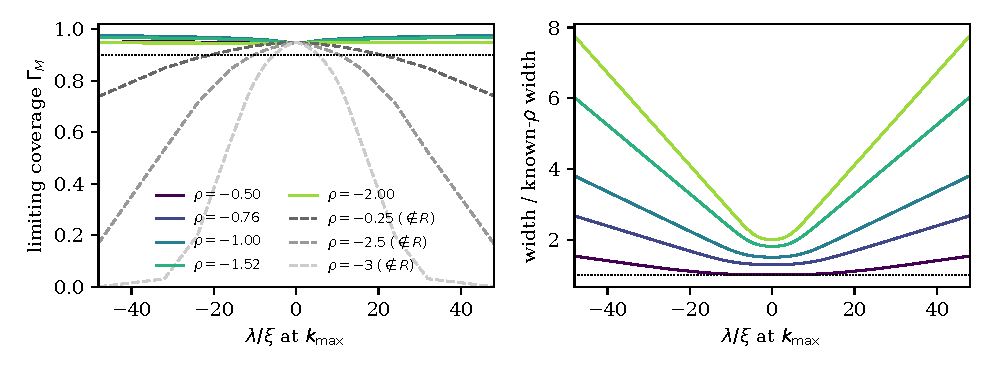
\includegraphics[width=\textwidth]{figures/limit_coverage_width.pdf}
\caption{Left: limiting simultaneous coverage $\Gamma_\Mesh(\rho,\lambda)$ of the six-point union band ($R=[-2,-0.5]$, nominal $0.90$, dotted) for $\rho$ inside $R$ (solid) and outside (dashed). Right: limiting mean width at $k_{\max}$ divided by the width of the known-$\rho$ band. Monte Carlo evaluation of the Gaussian limit in Theorem~\ref{thm:union}.}
\label{fig:limit}
\end{figure}

\paragraph{Width.} Theorem~\ref{thm:union}(f) separates four sources of width. The stochastic part is $G$, with variance $s_l^2$ per working value. The calibration constants $c_l$ depend on the grid through $(t_j)$ and $m$. The bias part $\mu_{jl}$ grows with $t_j$ and with $|\lambda|$. Uncertainty about $\rho$ enters through the hull over $l$: even at $\lambda=0$, the hull is at least as wide as the widest band, so $W_j\ge2\max_lc_ls_l$, and for $R=[-2,-0.5]$ the limiting mean width is up to \widthRatioZero{} times the width of the known-$\rho$ band (attained at $\rho=-2$, whose own band is narrowest). The ratio grows with $|\lambda|$ and reached \widthRatioMax{} at $|\lambda|/\xi=\lamMax$ in the evaluation of Remark~\ref{rem:numeric}. These are asymptotic statements; finite-sample widths are in Section~\ref{sec:sim}. The cost of not knowing $\rho$ is a bounded factor for bounded $|\lambda|$, not a factor that is uniform in $\lambda$.

\begin{corollary}[intersection over the grid]\label{cor:intersection}
Let $I=\bigcap_{j=1}^mU_j$. The events $\{\xi\in I\}$ and $\{\xi\in U_j\ \forall j\}$ are equal, so $\Prob(\xi\in I)\to\Gamma_\Mesh(\rho,\lambda)$, and $|I|\le\min_j|U_j|$. The set $I$ is the analogue, for our bands, of the snooping interval of \citet[eq.~15]{sasakiwang2024}. It can be empty; $\Prob(I=\emptyset)\le1-\Prob(\xi\in U_j\ \forall j)$.
\end{corollary}

The corollary does not say that intersections of valid intervals are valid in general; it uses that the bands are \emph{simultaneously} valid, and the intersection's coverage event is the simultaneous event itself. A user who reports $I$ only when it is non-empty has coverage $\Prob(\xi\in I)/\Prob(I\neq\emptyset)\ge\Prob(\xi\in I)$ conditional on reporting.

\begin{remark}[larger bias]\label{rem:R2}
If $\sqrt{k_j}\delta\{U(n/k_j)\}\to\pm\infty$ at a grid point, Theorem~\ref{thm:bvm} does not apply. If the centres at two mesh points $\rho_l<\rho<\rho_{l'}$ then satisfy a first-order bias expansion with remainder $o(\delta)$, the argument of Theorem~\ref{thm:union}(d) gives $\Prob(\xi\in U_j)\to1$. We do not prove that expansion. Extending the mesh slightly beyond $R$ would place every $\rho\in R$ strictly inside it; we did not do this in the method evaluated below.
\end{remark}

\section{Calibration and computation}\label{sec:computation}

\paragraph{Critical values.} Under exact Pareto tails the log-spacings above $X_{n-k_m,n}$ have the law of $\xi(\sum_{l=i}^{k_m}E_l/l)_{i\le k_m}$ with $E_l$ independent standard exponential \citep{renyi1953}, free of $n$, $C$ and, after division by $\xi$, of $\xi$. We compute $c(\rho_l)$ as the $(1-\alpha)$-quantile of $\max_j\sqrt{k_j}|\hat\xi_j(\rho_l)-1|/s(\rho_l)$ over simulated Pareto paths at the actual grid (1500 paths per working value). By Theorem~\ref{thm:bvm}(ii)--(iii) at $\lambda=0$ these quantiles converge to $c(\rho_l)$. At finite $k$ the endpoint constants of $U^+$ must control both tails separately, because the event bounded in Theorem~\ref{thm:uniform} is the upper exceedance at one endpoint and the lower at the other, and which is which depends on the sign of $\lambda$. We therefore take $c^+_l$, $l\in\{1,L\}$, as the larger of the $(1-\alpha/2)$-quantiles of $\max_j\sqrt{k_j}\{\hat\xi_j(\rho_l)-1\}/s(\rho_l)$ and of $\max_j\sqrt{k_j}\{1-\hat\xi_j(\rho_l)\}/s(\rho_l)$; in the limit both equal $c_l^+$. This is necessary because at finite $k$ the estimator is skewed: at $k\le1024$ under Pareto tails, the band at $\rho_1$ with its two-sided constant lies entirely above $\xi$ at some grid point with probability \finUp{} and entirely below with probability \finDn, against $\alpha/2$ each in the limit. The finite-$k$ upper-tail constant is accordingly up to \finOneFactor\% larger than the two-sided one, whereas in the limit the difference is about \widthOneSided\%. So at the sample sizes studied $U^+$ is a few per cent wider at the endpoint bands than $U$.

\begin{proposition}[exactness under Pareto tails]\label{prop:exact}
If $\bar F(x)=Cx^{-1/\xi}$ for $x\ge x_0$ and $c$ is the $(1-\alpha)$-quantile of $\max_j\sqrt{k_j}|\hat\xi_j(\rho')/\xi-1|/s(\rho')$ under exact Pareto tails at the same grid, then, conditionally on $X_{n-k_m,n}>x_0$, the pivot-inverted band
$\bigl[\hat\xi_j(\rho')/\{1+cs(\rho')k_j^{-1/2}\},\ \hat\xi_j(\rho')/\{1-cs(\rho')k_j^{-1/2}\}\bigr]$, $j=1,\dots,m$ (for $cs(\rho')<k_1^{1/2}$), has simultaneous coverage exactly $1-\alpha$.
\end{proposition}

The proof is the pivotality just described; Monte Carlo error in $c$ is the only approximation. The bands we compute, the posterior bands and the Wald band $\hat\xi_j\pm c\hat\xi_js/\sqrt{k_j}$, agree with this band to first order but not exactly, so no finite-sample statement is made for them, nor for second-order tails.

\paragraph{Posterior computation.} The posterior at a pair $(k,\rho')$ uses a prior under which $\log\xi$ is uniform on $[\log0.02,\log3]$ and $\delta$ is standard normal truncated to the valid region, and is computed by quadrature: 161 points in $\log\xi$ around the Hill estimate and 41 equal-probability nodes of the $\delta$ prior. This prior is not compactly supported in $\delta$ as Assumption~\ref{ass:P} requires, and quadrature with fixed resolution is a numerical approximation whose error is not controlled as $k\to\infty$; the theory concerns the exact posterior under a compactly supported prior.

\paragraph{Grid.} The evaluated method uses $k_{\max}=\lfloor n^{0.75}\rfloor$ and $k_j=\lfloor k_{\max}/2^{j}\rfloor$, $j=0,\dots,4$, fixed before seeing the data. Assumption~\ref{ass:A3} with finite $\lambda$ requires $k_{\max}\asymp n^{-2\rho/(1-2\rho)}$ or smaller, which is below $n^{0.75}$ when $\rho>-1.5$. The grid used in Section~\ref{sec:sim} is therefore not covered by the asymptotics for most of $R$; at the sample sizes studied, however, the realised values $|\lambda_j|/\xi$ were at most \lamBenchMax, and Section~\ref{sec:predict} checks whether the finite-$\lambda$ limit describes the results.

\paragraph{Mesh and reporting.} The mesh is six log-spaced points of $R=[-2,-0.5]$. Any $\hat k$ chosen from the data is mapped to the nearest grid point in $\log k$ and reported with $U_{\hat\jmath}$.

\section{Simulation study}\label{sec:sim}

\subsection{Design and disclosure}

The method, comparators, selection rules and decision thresholds were frozen and documented before a single confirmatory run on a previously unused seed. Families: Burr with $\rho\in\{-0.5,-1\}$, Fr\'echet ($\rho=-1$), the absolute value of a Student $t$ ($\rho=-2\xi$), each with $\xi\in\{0.5,1\}$ and $n\in\{2000,5000\}$, \benchReps{} replications per setting; and Burr with $\rho=-0.25$, outside $R$, reported but excluded from the decision rules. Methods: the union band; a plug-in band at an estimate $\hat\rho$; the first-order (Pareto) posterior band; the generalized Pareto posterior of \citet{dombry2023} with a pivotal band; and the frequentist twin of the plug-in band. Selection rules: SAMSEE, the rule of \citet{guillouhall2001}, a Lepski-type stability rule, and the largest grid point. Monte Carlo standard errors of coverages near $0.9$ are about \seBench.

\emph{Deviation from the pre-registration.} The protocol designated the plug-in band as primary and the union band as the robust variant. We lead with the union band because, after the confirmatory results were seen, the plug-in passed its decision rule with no margin and the analysis of Section~\ref{sec:rhohat} showed that its $\hat\rho$ did not estimate $\rho$. All pre-registered rules and results are reported unchanged. Sections~\ref{sec:predict}, \ref{sec:rhohat} and \ref{sec:comparators} are post hoc analyses; they use the same samples, regenerated from the same seed, or new development seeds, and change nothing in the evaluated method.

\subsection{Pre-registered results}

All four decision rules passed: the union band covered at least $0.85$ after all four selection rules in \DoneB{} of \nCellsIn{} settings (threshold \nCellsIn), the plug-in band in \DoneA{} (threshold 14), the first-order 90\% interval after the stability rule covered less than $0.80$ in \Dtwo{} (threshold 8), and the posterior plug-in band was closer to nominal simultaneous coverage than its frequentist twin in \Dthree{} (threshold 10). Table~\ref{tab:bench} gives the main coverages. Within the assumption the union band's simultaneous coverage was \unionSimIn{} and its smallest post-selection coverage \unionPostMinIn. Its 90\% interval at $k_{\max}$ was \unionVsPluginWidth{} times as wide as the plug-in's. The generalized Pareto band, whose validity requires the generalized Pareto approximation to be unbiased, had simultaneous coverage \gpSimIn. For Burr with $\rho=-0.25$ every method failed, including the union band (\unionSimOut).

\begin{table}[t]
\centering\small
\caption{Pre-registered benchmark: simultaneous coverage of the bands (sim.), smallest coverage of the band interval after the four selection rules (min post-sel.), and coverage of the first-order 90\% interval at the Lepski-selected $k$. Nominal 0.90; \benchReps{} replications; $^\dagger$ outside $R$.}
\label{tab:bench}
\setlength{\tabcolsep}{4pt}
\begin{tabular}{llrrrrrrrr}
\toprule
 & & & & \multicolumn{2}{c}{Union band} & \multicolumn{2}{c}{First-order} & \multicolumn{2}{c}{GP band}\\
\cmidrule(lr){5-6}\cmidrule(lr){7-8}\cmidrule(lr){9-10}
Family & $\rho$ & $\xi$ & $n$ & sim. & min post-sel. & sim. & Lepski int. & sim. & min post-sel.\\
\midrule
$|t|$ & $-2$ & 1 & 2000 & 0.97 & 0.98 & 0.90 & 0.86 & 0.93 & 0.97\\
$|t|$ & $-2$ & 1 & 5000 & 0.97 & 0.98 & 0.88 & 0.88 & 0.89 & 0.96\\
$|t|$ & $-1$ & 0.5 & 2000 & 0.97 & 0.99 & 0.50 & 0.33 & 0.89 & 0.96\\
$|t|$ & $-1$ & 0.5 & 5000 & 0.95 & 0.98 & 0.43 & 0.28 & 0.91 & 0.97\\
Burr & $-1$ & 0.5 & 2000 & 0.96 & 0.98 & 0.75 & 0.61 & 0.87 & 0.95\\
Burr & $-1$ & 0.5 & 5000 & 0.95 & 0.98 & 0.76 & 0.59 & 0.90 & 0.95\\
Burr & $-1$ & 1 & 2000 & 1.00 & 1.00 & 0.77 & 0.65 & 0.94 & 0.98\\
Burr & $-1$ & 1 & 5000 & 0.97 & 0.99 & 0.66 & 0.52 & 0.90 & 0.96\\
Burr & $-0.5$ & 0.5 & 2000 & 0.93 & 0.96 & 0.00 & 0.03 & 0.91 & 0.96\\
Burr & $-0.5$ & 0.5 & 5000 & 0.92 & 0.95 & 0.00 & 0.05 & 0.91 & 0.95\\
Burr & $-0.5$ & 1 & 2000 & 0.97 & 0.98 & 0.00 & 0.03 & 0.83 & 0.84\\
Burr & $-0.5$ & 1 & 5000 & 0.97 & 0.98 & 0.00 & 0.03 & 0.71 & 0.77\\
Fr\'echet & $-1$ & 0.5 & 2000 & 0.96 & 0.99 & 0.86 & 0.84 & 0.90 & 0.97\\
Fr\'echet & $-1$ & 0.5 & 5000 & 0.97 & 0.99 & 0.88 & 0.79 & 0.93 & 0.98\\
Fr\'echet & $-1$ & 1 & 2000 & 0.97 & 0.98 & 0.86 & 0.83 & 0.89 & 0.96\\
Fr\'echet & $-1$ & 1 & 5000 & 0.97 & 0.98 & 0.84 & 0.78 & 0.91 & 0.96\\
Burr$^{\dagger}$ & $-0.25$ & 0.5 & 2000 & 0.24 & 0.30 & 0.00 & 0.01 & 0.47 & 0.50\\
Burr$^{\dagger}$ & $-0.25$ & 0.5 & 5000 & 0.15 & 0.17 & 0.00 & 0.00 & 0.23 & 0.25\\
Burr$^{\dagger}$ & $-0.25$ & 1 & 2000 & 0.77 & 0.78 & 0.00 & 0.00 & 0.00 & 0.00\\
Burr$^{\dagger}$ & $-0.25$ & 1 & 5000 & 0.79 & 0.82 & 0.00 & 0.00 & 0.00 & 0.00\\
\bottomrule
\end{tabular}

\end{table}

\subsection{Does the limit theory predict the coverage?}\label{sec:predict}

For each setting we computed $\Gamma_\Mesh$ at the setting's own grid, with $\lambda_j=\sqrt{k_j}\,\delta\{U(n/k_j)\}$ obtained exactly from the family's survival function through Assumption~\ref{ass:A1}, and with $G$ replaced by the estimators simulated under exact Pareto tails at that grid. This is a finite-$k$ approximation of $\Gamma_\Mesh$, not the Gaussian limit itself. Within the assumption the predictions were \predIn{} and the observed coverages \obsIn; the differences were \diffIn{} (Figure~\ref{fig:predict}). This includes settings whose largest grid point had $|\lambda_j|/\xi$ up to \lamBenchMax. For Burr with $\rho=-0.25$ the prediction (\predOut) failed: the observed coverage was \obsOut. There $|\delta\{U(n/k_{\max})\}|/\xi$ was \deltaRatioOut, so the second-order term was as large as the Pareto term and the local expansion behind Theorem~\ref{thm:bvm} did not apply; within the assumption the same ratio was at most \deltaRatioIn. The failure at $\rho=-0.25$ is therefore not explained by $\rho\notin R$, which the limit would tolerate at these $\lambda$, but by the breakdown of the local regime.

\begin{figure}[t]
\centering
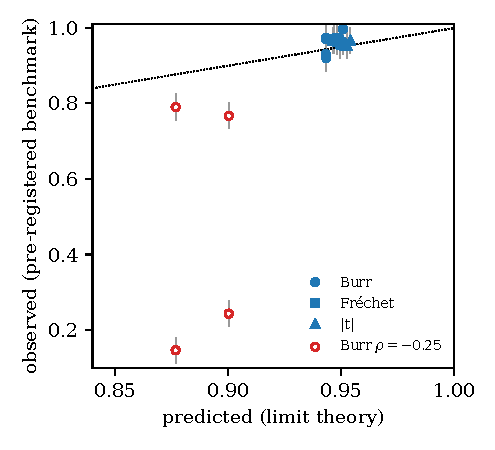
\includegraphics[width=0.5\textwidth]{figures/predicted_vs_observed.pdf}
\caption{Simultaneous coverage of the union band: finite-$k$ approximation of $\Gamma_\Mesh$ at each setting's grid and exact $\lambda_j$ (horizontal) against the pre-registered benchmark (vertical, bars $\pm2$ Monte Carlo standard errors). Open markers: Burr $\rho=-0.25$.}
\label{fig:predict}
\end{figure}

\subsection{The plug-in estimate of \texorpdfstring{$\rho$}{rho}}\label{sec:rhohat}

The frozen plug-in used the statistic $T$ of \citet{fagh2003} in the form $\hat\rho=-|3(T-1)/(T-3)|$ of \citet{cgp2005}, at $k_1=\lfloor n^{0.999}\rfloor$, switching from $\tau=0$ to $\tau=1$ whenever the $\tau=0$ value was below $-1$. This differs from \citet{cgp2005}, who use $k_1=\min(n-1,\lfloor2n^{0.995}/\log\log n\rfloor)$ and choose $\tau$ by the region of $\rho$. In a separate check (development seed, $\xi=0.5$, $n$ up to $10^6$) the $\tau=0$ value at $k_1=n^{0.999}$ was nearly constant across replications but not near $\rho$: medians \rhoNineNineNineBurrA, \rhoNineNineNineBurrB{} and \rhoNineNineNineBurrC{} for Burr with $\rho=-0.25,-0.5,-1$ at $n=10^6$. The switch to $\tau=1$ produced \rhoFrechetSwitch{} for the Fr\'echet distribution ($\rho=-1$). With $\tau=0$ and $k_1=n^{0.9}$ the estimate approached $\rho$ at $n=10^6$ (\rhoNineBurrC{} for Burr $\rho=-1$, \rhoNineFrechet{} for Fr\'echet, \rhoNineBurrB{} for Burr $\rho=-0.5$) but was noisy at $n=5000$ (Burr $\rho=-1$: median \rhoNineBurrCsmall) and still \rhoNineBurrA{} for Burr $\rho=-0.25$. The supported conclusion is limited to this: at a few thousand observations no single $k_1$ gave a reliable $\hat\rho$ across $R$. Lemma~\ref{lem:beta} quantifies what a plug-in at an inconsistent $\hat\rho$ with limit $\rho'$ leaves: for $\rho'=-0.76$ and $\rho=-0.5$, $27\%$ of the Hill bias.

\subsection{Additional comparators (post hoc)}\label{sec:comparators}

We evaluated two further comparators on the same samples. The first is the interval $H^O$ of \citet[eq.~11]{sasakiwang2024} at a deterministic threshold: the Hill estimate plus or minus $(z_{0.95}\hat\xi+\bar B)/\sqrt{k}$ with their rule-of-thumb bias bound, which makes the bias allowance $0.1\hat\xi$. We report its pointwise coverage at $k_{\max}$ and, as a description of the practice they recommend, its coverage at the grid point nearest to the Guillou--Hall choice (critical value 1.25, as in their implementation). We also evaluated their snooping interval $H^S$ \citep[eq.~15]{sasakiwang2024}, the intersection of $H^O$ over our five grid points with their tabulated critical value $2.67$ for 90\% and $\underline r=1/20$, which is conservative for our grid ratio of $1/16$. Their text writes the rule-of-thumb bound with $\sqrt{r\bar k}$; we read $r\bar k$ as the threshold $k_j$ at which each interval is computed, so the bias allowance is again $0.1\hat\xi_j$. This comparison is between methods with different assumptions: their interval is valid uniformly over a class defined by $(A,\rho)$, ours pointwise under $\rho\in R$. The second comparator is the plug-in band with $\hat\rho$ computed as in \citet{cgp2005}, giving it the favourable choice of $\tau$ by the true region of $\rho$. Within the assumption, the Sasaki--Wang interval at $k_{\max}$ covered at least \swTopGoodMin{} except for Burr with $\rho=-0.5$, where the Hill bias exceeds its bias allowance and coverage was \swTopBurr; at the Guillou--Hall threshold it covered \swGHIn. Its width at $k_{\max}$ was \swWidthRatio{} times that of the union band, but it is a pointwise interval and the union band a simultaneous band, so the widths are not like for like. Their snooping interval, which is simultaneous like ours, covered \swSnoopGood{} in the same settings and \swSnoopBurr{} for Burr with $\rho=-0.5$ (\swSnoopOut{} for $\rho=-0.25$); its median width was \swSnoopWidthRatio{} times that of the intersection of our union bands. Its failures reflect the rule-of-thumb bound, which a user could enlarge; ours reflect the range $R$, which a user could widen at a cost in width. The corrected plug-in band had simultaneous coverage \cgpSimIn{} (at least $0.85$ in \cgpSimInN{} of \nCellsIn{} settings). Table~\ref{tab:posthoc} gives all settings.

\begin{table}[t]
\centering\small
\caption{Post hoc comparators on the confirmatory samples: Sasaki--Wang interval $H^O$ with their rule-of-thumb bias bound (pointwise coverage at $k_{\max}$, coverage at the Guillou--Hall threshold, mean width at $k_{\max}$), plug-in band with the $\hat\rho$ of \citet{cgp2005}, and the union band. Widths are of the band at $k_{\max}$. $^\dagger$ outside $R$.}
\label{tab:posthoc}
\setlength{\tabcolsep}{3.5pt}\footnotesize
\begin{tabular}{llrrrrrrrrr}
\toprule
 & & & & \multicolumn{3}{c}{Sasaki--Wang $H^{O}$ (pointwise)} & \multicolumn{2}{c}{CGP plug-in band} & \multicolumn{2}{c}{Union band}\\
\cmidrule(lr){5-7}\cmidrule(lr){8-9}\cmidrule(lr){10-11}
Family & $\rho$ & $\xi$ & $n$ & cov.\ $k_{\max}$ & after GH & width $k_{\max}$ & sim. & width $k_{\max}$ & sim. & width $k_{\max}$\\
\midrule
$|t|$ & $-2$ & 1 & 2000 & 1.00 & 0.96 & 0.395 & 0.91 & 0.395 & 0.97 & 0.609\\
$|t|$ & $-2$ & 1 & 5000 & 1.00 & 0.96 & 0.338 & 0.89 & 0.277 & 0.97 & 0.470\\
$|t|$ & $-1$ & 0.5 & 2000 & 0.98 & 0.94 & 0.220 & 0.92 & 0.289 & 0.97 & 0.348\\
$|t|$ & $-1$ & 0.5 & 5000 & 1.00 & 0.98 & 0.184 & 0.93 & 0.200 & 0.95 & 0.249\\
Burr & $-1$ & 0.5 & 2000 & 0.99 & 0.92 & 0.211 & 0.91 & 0.282 & 0.96 & 0.353\\
Burr & $-1$ & 0.5 & 5000 & 1.00 & 0.97 & 0.178 & 0.91 & 0.191 & 0.95 & 0.255\\
Burr & $-1$ & 1 & 2000 & 1.00 & 0.95 & 0.421 & 0.94 & 0.529 & 1.00 & 0.638\\
Burr & $-1$ & 1 & 5000 & 1.00 & 0.96 & 0.357 & 0.92 & 0.377 & 0.97 & 0.487\\
Burr & $-0.5$ & 0.5 & 2000 & 0.06 & 0.81 & 0.265 & 0.80 & 0.291 & 0.93 & 0.371\\
Burr & $-0.5$ & 0.5 & 5000 & 0.02 & 0.86 & 0.220 & 0.76 & 0.203 & 0.92 & 0.269\\
Burr & $-0.5$ & 1 & 2000 & 0.02 & 0.81 & 0.534 & 0.86 & 0.622 & 0.97 & 0.820\\
Burr & $-0.5$ & 1 & 5000 & 0.00 & 0.89 & 0.442 & 0.86 & 0.440 & 0.97 & 0.614\\
Fr\'echet & $-1$ & 0.5 & 2000 & 1.00 & 0.96 & 0.204 & 0.90 & 0.247 & 0.96 & 0.357\\
Fr\'echet & $-1$ & 0.5 & 5000 & 1.00 & 0.96 & 0.173 & 0.89 & 0.169 & 0.97 & 0.262\\
Fr\'echet & $-1$ & 1 & 2000 & 1.00 & 0.96 & 0.408 & 0.87 & 0.468 & 0.97 & 0.624\\
Fr\'echet & $-1$ & 1 & 5000 & 1.00 & 0.97 & 0.346 & 0.92 & 0.334 & 0.97 & 0.479\\
Burr$^{\dagger}$ & $-0.25$ & 0.5 & 2000 & 0.00 & 0.62 & 0.404 & 0.00 & 0.370 & 0.24 & 0.553\\
Burr$^{\dagger}$ & $-0.25$ & 0.5 & 5000 & 0.00 & 0.62 & 0.325 & 0.00 & 0.248 & 0.15 & 0.420\\
Burr$^{\dagger}$ & $-0.25$ & 1 & 2000 & 0.00 & 0.58 & 0.806 & 0.36 & 0.960 & 0.77 & 1.395\\
Burr$^{\dagger}$ & $-0.25$ & 1 & 5000 & 0.00 & 0.62 & 0.650 & 0.32 & 0.640 & 0.79 & 1.101\\
\bottomrule
\end{tabular}

\end{table}


\section{Application: Danish fire insurance losses}\label{sec:danish}

The data are $n=\danishN$ large fire insurance claims \citep{mcneil1997}, read at run time from the R package \texttt{evir}; no data are redistributed with this paper. The frozen method was applied unchanged with grid $\{\danishKs\}$. SAMSEE and the Guillou--Hall rule chose $k=\danishSamsee$ and $k=\danishGH$, which map to grid points \danishKsam{} and \danishKgh. Table~\ref{tab:danish} and Figure~\ref{fig:danish} give the bands. Reporting $U_j$ at either selected grid point carries the guarantee of Theorem~\ref{thm:union}(c); reporting the first-order 90\% interval at the selected $k$ does not. The intersection of the union bands over the grid is \danishInter{} (Corollary~\ref{cor:intersection}). The claims arrive irregularly over time, and independence is a conventional assumption here, not a verified one.

\begin{table}[t]
\centering\small
\caption{Danish fire losses: band intervals at each grid point and first-order 90\% interval.}
\label{tab:danish}
\begin{tabular}{rcccc}
\toprule
$k$ & Union band & First-order band & GP band & First-order 90\% int.\\
\midrule
19 & [0.365, 1.587] & [0.380, 1.053] & [0.247, 2.597] & [0.424, 0.909]\\
39 & [0.379, 1.295] & [0.398, 0.806] & [0.302, 1.679] & [0.431, 0.731]\\
79 & [0.364, 1.009] & [0.467, 0.765] & [0.268, 1.026] & [0.494, 0.716]\\
158 & [0.379, 0.843] & [0.616, 0.873] & [0.261, 0.767] & [0.642, 0.834]\\
317 & [0.523, 0.976] & [0.619, 0.792] & [0.490, 0.939] & [0.638, 0.767]\\
\midrule
$\cap_j$ & [0.523, 0.843] & & & \\
\bottomrule
\end{tabular}

\end{table}

\begin{figure}[t]
\centering
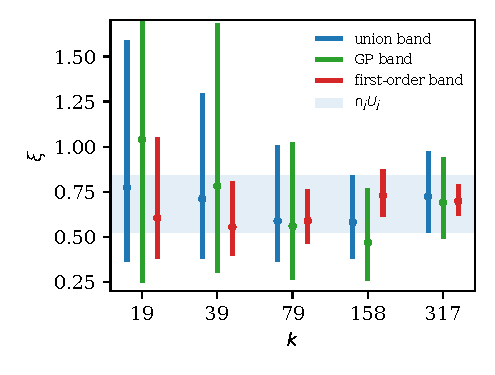
\includegraphics[width=0.5\textwidth]{figures/danish.pdf}
\caption{Danish fire losses: bands along the grid (posterior medians as dots) and the intersection of the union bands (shaded). Bands extending beyond the plotted range are clipped (\danishClip; Table~\ref{tab:danish}).}
\label{fig:danish}
\end{figure}

\section{Discussion and limitations}\label{sec:discussion}

The construction gives up adaptive length: \citet{carpentierkim2014} show that honest adaptive intervals need a separation condition, and \citet{sasakiwang2024} bound the expected length of uniformly valid intervals from below by a worst-case bias modulus. It gains, in exchange, for validity after any data-driven choice of $k$ on a fixed grid, and it replaces the estimability of $\rho$ by membership of $\rho$ in a stated range. The union device is classical. What makes a coarse mesh work here is that the bias at a wrong working value changes sign at the true value, so the mesh brackets every $\rho$ inside it; a similar sign change of the residual bias appears for generalized jackknife estimators computed at a fixed $\rho$ \citep{gomesmartinsneves2002}. The same sign change gives the coverage bound of Theorem~\ref{thm:uniform}, which uses only the two endpoint bands. At the sample sizes simulated, the finite-$k$ approximation of the limit was within \diffAbsMax{} of the observed coverage in the settings within the assumption, though it explains little of the variation between settings and it failed for Burr with $\rho=-0.25$.

The limitations are as follows.
\begin{enumerate}
\item All guarantees are pointwise asymptotic: uniform over $\rho\in R$ and $\lambda\in\R$ for the limit, but not uniform in $F$ for fixed $n$. Coverage at least $1-\alpha$ on all of $R$ is proved for the endpoint-calibrated band $U^+$; for the band evaluated in Section~\ref{sec:sim}, which uses two-sided constants, the proved bound is $1-\varphi_\Mesh$ (\boundTwo{} for our mesh, to Monte Carlo accuracy), and the numerically computed minimum \GammaMinR{} is not a theorem. $U^+$ was derived after the confirmatory study and was not evaluated in it. Nothing is exact under second-order tails.
\item The width keeps the rate $k^{-1/2}$ for each fixed $\lambda$, but the constant grows linearly in $|\lambda|$, and at $\lambda=0$ it is up to \widthRatioZero{} times the known-$\rho$ width.
\item The theory is local. When the second-order term is as large as the Pareto term, as for Burr $\rho=-0.25$ at the top of our grid, no method we tried covered, and the limit did not predict this. Remark~\ref{rem:R2} extends validity only under an unproved expansion.
\item The grid rule $k_{\max}=\lfloor n^{0.75}\rfloor$ is asymptotically outside the local regime for $\rho>-1.5$; agreement with the limit at the sample sizes studied is evidence, not a theorem.
\item Assumptions~\ref{ass:A2} and \ref{ass:P} are not verified for the families simulated or for the implemented prior and quadrature.
\item The union band is conservative. Multiplying all critical values by $0.90$ would give a worst-case limiting coverage of \kappaWorst{} over the evaluated range, with correspondingly narrower bands; we did not adopt this, because it would change the method after the confirmatory study.
\item The pre-registered plug-in comparator used a non-standard $\hat\rho$ recipe (Section~\ref{sec:rhohat}).
\end{enumerate}

Open problems include whether $\Gamma_\Mesh\ge1-\alpha$ on $R$ for the two-sided calibration, a version of Theorem~\ref{thm:uniform} uniform over a class of distributions at finite $n$, a lower bound on the width of any band with post-selection coverage over $R$, a data-driven upper end of the grid, and a data-informed choice of $R$.

\paragraph{Reproducibility.} The code, the frozen benchmark code with its source hashes, the raw simulation outputs and the scripts that generate every number, table and figure of this paper are in the repository \url{https://github.com/EllenSyuu/tailfm-union-band}; release \texttt{v1.0.0}, archived at \url{https://doi.org/10.5281/zenodo.24022373}, corresponds to this version of the paper. All numerical statements in the text are generated from stored outputs.

\bibliographystyle{plainnat}
\bibliography{references}

\appendix
\section{Proofs}\label{app:proofs}

Throughout, $K=k_m$ is the largest grid point. Exact Pareto tails ($\delta\equiv0$) are not
in the class of Assumption~\ref{ass:A1}; wherever we argue ``under $p^{\otimes K}$'' the argument is
for exact Pareto excesses directly and does not use Assumption~\ref{ass:A1}. Further, $E\sim\mathrm{Exp}(1)$, and for $s<1$ we use
$\E e^{sE}=(1-s)^{-1}$ and $\E(Ee^{sE})=(1-s)^{-2}$.

\subsection{Scores, efficiency and the bias factor}

\begin{lemma}\label{lem:scores}
Let $Y$ have the EPD$(\xi,\delta;\rho')$ distribution and $E=\xi^{-1}\log Y$. At $\delta=0$:
\begin{enumerate}
\item[(i)] the scores for $(\xi,\delta)$ are $\xi^{-1}(E-1)$ and $\xi^{-1}a_{\rho'}(E)$, with
$a_{\rho'}(E)=(1-\rho')e^{\rho'E}-1$, and the Fisher information is
$\xi^{-2}\begin{pmatrix}1&c'\\c'&d'\end{pmatrix}$ with $c'=\rho'/(1-\rho')$,
$d'=\rho'^2/(1-2\rho')$; its determinant is $\xi^{-4}\rho'^4/\{(1-2\rho')(1-\rho')^2\}>0$;
\item[(ii)] the efficient influence function for $\xi$ is $\xi\psi_{\rho'}(E)$ with $\psi_{\rho'}$
as in Section~\ref{sec:bvm}, $\E\psi_{\rho'}(E)=0$ and $\operatorname{var}\psi_{\rho'}(E)=s(\rho')^2$;
\item[(iii)] differentiating $y^{-1/\xi}\{1+\xi^{-1}\delta(y^{\rho/\xi}-1)\}$, the conditional
survival function implied by Assumption~\ref{ass:A1} to first order in $\delta$, at
$\delta=0$ gives the log-density derivative $h_\rho$ of \eqref{eq:h}, and
$h_\rho(Y)=\xi^{-1}a_\rho(E)$;
\item[(iv)] $\operatorname{cov}\{\psi_{\rho'}(E),a_\rho(E)\}=\beta(\rho,\rho')$ and
$\operatorname{cov}\{E-1,a_\rho(E)\}=\rho/(1-\rho)$;
\item[(v)] under exact Pareto excesses, the estimator of \citet{bjs2009} at the working
value $\rho'$ satisfies $\sqrt{k}\{\hat\xi(\rho')-\xi\}/\xi=k^{-1/2}\sum_{i\le k}\psi_{\rho'}(E_i)+o_P(1)$.
\end{enumerate}
\end{lemma}

\begin{proof}
(i) The EPD log-density at $\delta=0$ is the Pareto log-density, whose $\xi$-score is
$\xi^{-1}(E-1)$; the dependence of $\rho'/\xi$ on $\xi$ does not enter at $\delta=0$.
Differentiating the EPD log-density in $\delta$ at $\delta=0$ gives $\xi^{-1}a_{\rho'}(E)$.
The moments $\operatorname{var}(E)=1$, $\operatorname{cov}(E,a_{\rho'})=\rho'/(1-\rho')$ and
$\operatorname{var}(a_{\rho'})=\rho'^2/(1-2\rho')$ follow from the two exponential moments.
(ii) The efficient influence function is the first row of the inverse information applied to
the scores: $\xi\{d'(E-1)-c'a_{\rho'}(E)\}/(d'-c'^2)$, and
$d'/(d'-c'^2)=(1-\rho')^2/\rho'^2$, $c'/(d'-c'^2)=(1-2\rho')(1-\rho')/\rho'^3$. Its variance is
$\xi^2d'/(d'-c'^2)=\xi^2s(\rho')^2$.
(iii) Direct differentiation; with $y=e^{\xi E}$ the result is $\xi^{-1}\{(1-\rho)e^{\rho E}-1\}$.
(iv) $\operatorname{cov}(a_{\rho'},a_\rho)=\rho\rho'/(1-\rho-\rho')$, and
$\{d'\rho/(1-\rho)-c'\rho\rho'/(1-\rho-\rho')\}/(d'-c'^2)=\beta(\rho,\rho')$ by the identity
$(1-\rho')(1-\rho-\rho')-(1-2\rho')(1-\rho)=\rho'(\rho'-\rho)$.
(v) The estimator is $\hat\xi=H-\hat\delta\rho'/(1-\rho')$ with $H=k^{-1}\sum\xi E_i$,
$\hat\delta=H(1-2\rho')(1-\rho')^3\rho'^{-4}\{M-(1-\rho')^{-1}\}$ and
$M=k^{-1}\sum\exp(\rho'\xi E_i/H)$. Under exact Pareto excesses the $E_i$ are independent
standard exponential and $\varepsilon=H/\xi-1=O_P(k^{-1/2})$. Write
$M=k^{-1}\sum f(E_i,\varepsilon)$ with $f(e,t)=\exp\{\rho'e/(1+t)\}$. As $\rho'<0$ and $e\ge0$,
$|\partial_t^2f(e,t)|\le C(e+e^2)$ for $|t|\le1/2$, so
$M=k^{-1}\sum e^{\rho'E_i}-\varepsilon\rho'k^{-1}\sum E_ie^{\rho'E_i}+O_P(k^{-1})$.
Up to $o_P(k^{-1/2})$, $\hat\xi$ is therefore a smooth function of three sample means with finite
variances, and the delta method gives an asymptotically linear expansion whose
influence function, after the algebra, equals $\psi_{\rho'}$. \qedhere
\end{proof}

\begin{proof}[Proof of Lemma~\ref{lem:beta}]
All factors of $\beta$ other than $\rho'-\rho$ are positive or pair to the positive ratio
$\rho/\rho'$. The Hill ratio follows from (iv): the Hill estimator has influence $E-1$, so its
bias is $\lambda\rho/(1-\rho)$ by the argument of Theorem~\ref{thm:bvm}(ii). \qedhere
\end{proof}

\begin{lemma}\label{lem:suff}
If $q_u/p=1+\delta(u)h_\rho+r_u$ with $\sup_{y\ge1}|r_u(y)|y^{-\epsilon}=o\{\delta(u)\}$ for some
$\epsilon<1/(4\xi)$, then Assumption~\ref{ass:A2} holds.
\end{lemma}

\begin{proof}
Let $v=\delta h_\rho+r_u\ge-1$ and $g(v)=(1+v)^{1/2}-1-v/2$, so that $|g(v)|\le v^2/2$ for
$v\ge-1$. The integrand of Assumption~\ref{ass:A2} is $p\{g(v)+r_u/2\}^2\le2pg(v)^2+pr_u^2/2$.
Since $h_\rho$ is bounded on $[1,\infty)$ and $\int y^{4\epsilon}p(y)\,dy<\infty$ for
$4\epsilon<1/\xi$, $\int pr_u^2=o(\delta^2)$ and
$\int pg(v)^2\le\frac14\int pv^4\le2\int p(\delta^4h_\rho^4+r_u^4)=o(\delta^2)$. \qedhere
\end{proof}

\subsection{Joint limits under Pareto tails}

\begin{lemma}\label{lem:clt}
Let $E_1,\dots,E_K$ be independent standard exponential and, for $j\le m$ and $i\le k_j$,
$V^{(j)}_i=\sum_{l=i}^{k_j}E_l/l$. For functions $\phi$ with $\E\phi(E)=0$, $\E\phi(E)^2<\infty$ and
$\phi',\phi''$ bounded on $[0,\infty)$, put $S_j(\phi)=k_j^{-1/2}\sum_{i\le k_j}\phi(V^{(j)}_i)$.
Then for finitely many such pairs $(j,\phi)$ the vector of the $S_j(\phi)$ is asymptotically
centred normal, and for two such functions $\phi,\chi$ and $t_j\le t_{j'}$,
$\lim\operatorname{cov}\{S_j(\phi),S_{j'}(\chi)\}=(t_j/t_{j'})^{1/2}\operatorname{cov}\{\phi(E),\chi(E+\log(t_{j'}/t_j))\}$.
\end{lemma}

Under exact Pareto excesses above $X_{n-K,n}$, R\'enyi's representation gives
\[
\xi^{-1}\log(X_{n-i+1,n}/X_{n-k_j,n})=V^{(j)}_i\qquad(i\le k_j\le K)
\]
jointly, with the same $E_l$, namely the normalised spacings $l\,\xi^{-1}\log(X_{n-l+1,n}/X_{n-l,n})$.
So every statistic $k_j^{-1/2}\sum_{i\le k_j}\phi\{\xi^{-1}\log(X_{n-i+1,n}/X_{n-k_j,n})\}$ equals
$S_j(\phi)$ in law, jointly in $j$ and $\phi$. The functions $\psi_{\rho'}$ and $a_\rho$ satisfy the conditions of the
lemma, because $\rho,\rho'<0$ make $e^{\rho z}$ and its derivatives bounded on $[0,\infty)$.

\begin{proof}
\emph{Linearisation.} Fix $j$ and write $r_i=\sum_{l=i}^{k_j}1/l=\E V^{(j)}_i$ and
$V^{(j)}_i-r_i=\sum_{l=i}^{k_j}(E_l-1)/l$, so that $\E(V^{(j)}_i-r_i)^2=\sum_{l\ge i}l^{-2}\le2/i$.
Taylor's theorem with $|\phi''|\le C$ gives
\[
S_j(\phi)=k_j^{-1/2}\sum_{i\le k_j}\phi(r_i)+k_j^{-1/2}\sum_{l\le k_j}w_{jl}(E_l-1)+R_j,\qquad
w_{jl}=\frac1l\sum_{i\le l}\phi'(r_i),
\]
with $|R_j|\le Ck_j^{-1/2}\sum_{i\le k_j}(V^{(j)}_i-r_i)^2$. Since
$\E(V^{(j)}_i-r_i)^4\le9(\sum_{l\ge i}l^{-2})^2\le36/i^2$, Minkowski's inequality gives
$(\E R_j^2)^{1/2}\le Ck_j^{-1/2}\sum_{i\le k_j}6/i=O(k_j^{-1/2}\log k_j)\to0$. The weights satisfy
$|w_{jl}|\le\sup|\phi'|$. The deterministic term is a Riemann sum: $r_i=\log(k_j/i)+O(1/i)$,
so $k_j^{-1}\sum_{i\le k_j}\phi(r_i)=\int_0^1\phi(-\log s)\,ds+O(k_j^{-1}\log k_j)$, using
$|\phi(r_i)-\phi(\log(k_j/i))|\le C/i$ and the monotone comparison of the sum with the integral
for the function $s\mapsto\phi(-\log s)$, whose variation on $[1/k_j,1]$ is $O(\log k_j)$, together with
$\int_0^{1/k_j}|\phi(-\log s)|\,ds=O(k_j^{-1}\log k_j)$, as $|\phi(z)|\le C(1+z)$. Since
$\int_0^1\phi(-\log s)\,ds=\E\phi(E)=0$, the deterministic term is $O(k_j^{-1/2}\log k_j)\to0$.

\emph{Joint normality.} Hence, up to $o_P(1)$, every $S_j(\phi)$ is a linear form
$\sum_{l\le K}c^{(n)}_{l}(E_l-1)$ in the same independent variables with coefficients bounded by
$C k^{-1/2}$. For any fixed linear combination of finitely many such forms, the coefficients are
again $O(k^{-1/2})$, so the Lindeberg condition holds and the Lindeberg--Feller theorem gives
asymptotic normality of the combination, provided its variance converges; the Cram\'er--Wold
device then gives joint asymptotic normality. Since the remainders and the deterministic terms
vanish in $L^2$, the variance of each combination differs by $o(1)$ from that of the same
combination of the $S_j(\phi)$, which converges by the covariance computation below.

\emph{Covariance.} Let $j<j'$. The excesses $\{V^{(j)}_i\}_{i\le k_j}$ are functions of
$E_1,\dots,E_{k_j}$, and $V^{(j')}_i=V^{(j)}_i+D$ for $i\le k_j$ with $D=\sum_{l=k_j+1}^{k_{j'}}E_l/l$,
while $V^{(j')}_i$ for $k_j<i\le k_{j'}$ depends only on $E_{k_j+1},\dots,E_{k_{j'}}$. Hence
$S_j(\phi)$ is independent of $D$ and of the second group, and
\[
\operatorname{cov}\{S_j(\phi),S_{j'}(\chi)\}=(k_jk_{j'})^{-1/2}\,\E_D\Bigl[\operatorname{cov}\Bigl\{\textstyle\sum_{i\le k_j}\phi(V^{(j)}_i),\sum_{i\le k_j}\chi(V^{(j)}_i+D)\Bigm|D\Bigr\}\Bigr].
\]
The multiset $\{V^{(j)}_i\}_{i\le k_j}$ has the law of an independent sample of $k_j$ standard
exponentials (R\'enyi), and both sums are symmetric functions of it, so the conditional
covariance equals $k_j\operatorname{cov}\{\phi(E),\chi(E+D)\}$ evaluated at the realised $D$. As
$D\to\log(k_{j'}/k_j)\to\log(t_{j'}/t_j)$ in probability and the map
$d\mapsto\operatorname{cov}\{\phi(E),\chi(E+d)\}$ is bounded and continuous (by the bounds on
$\chi'$), dominated convergence gives the stated limit. The case $j=j'$ gives
$\operatorname{var}S_j(\phi)=\operatorname{var}\phi(E)$ exactly. \qedhere
\end{proof}

\subsection{Local asymptotic normality}

Let $D^{(m)}=(X_{n-i+1,n}/X_{n-K,n})_{i\le K}$, taken in random order. Every statistic used in
this paper, at every grid point and working value, is a function of $D^{(m)}$. Given
$X_{n-K,n}=u$, $D^{(m)}$ is an independent sample from $q_u$; under exact Pareto tails it is an
independent sample from $p$.

\begin{lemma}\label{lem:lan}
Assume \ref{ass:A1}--\ref{ass:A3}. For any deterministic sequence $u_n$ with
$\sqrt{K}\,\delta(u_n)\to\lambda_m=\lambda$, the log-likelihood ratio of $q_{u_n}^{\otimes K}$
with respect to $p^{\otimes K}$ satisfies, under $p^{\otimes K}$,
$\log\prod_{i\le K}(q_{u_n}/p)(Y_i)=\lambda\Delta_K-\tfrac12\lambda^2\sigma_h^2+o_P(1)$, with
$\Delta_K=K^{-1/2}\sum_{i\le K}h_\rho(Y_i)\dto N(0,\sigma_h^2)$ and $\sigma_h^2=\int h_\rho^2p=\xi^{-2}\rho^2/(1-2\rho)$. The two
sequences of laws are mutually contiguous.
\end{lemma}

\begin{proof}
Put $\eta_n=\delta(u_n)$ and $W_{i}=2\{(q_{u_n}/p)^{1/2}(Y_i)-1\}$. The function $h_\rho$ satisfies $\int h_\rho p=0$ and $\int h_\rho^2p<\infty$. Both $q_{u_n}$ and $p$ are densities on $[1,\infty)$ and $p>0$ there, so $q_{u_n}$ is absolutely continuous with respect to $p$ and the likelihood ratio $q_{u_n}/p$ is well defined; we do not assume the converse, since $q_{u_n}$ may vanish on part of $[1,\infty)$. On $N_n=\{q_{u_n}=0\}$ the integrand of Assumption~\ref{ass:A2} equals $p(1+\frac12\eta_nh_\rho)^2\ge p/4$ for $n$ large, because $h_\rho$ is bounded; hence $\int_{N_n}p=o(\eta_n^2)$, and the probability under $p^{\otimes K}$ that some $Y_i$ falls in $N_n$ is at most $K\int_{N_n}p=o(K\eta_n^2)=o(1)$. So with probability tending to one every $W_i>-2$ and the log-likelihood ratio below is finite. The argument in the proof of Theorem~7.2 of \citet{vandervaart1998} uses only the expansion
$\int\{q_n^{1/2}-p^{1/2}-\frac12\eta_nh\,p^{1/2}\}^2=o(\eta_n^2)$ along the sequence and
$\sqrt{K}\eta_n\to\lambda$, and yields $\sum_iW_i=\lambda\Delta_K-\lambda^2\sigma_h^2/4+o_P(1)$,
$\sum_iW_i^2\to\lambda^2\sigma_h^2$ in probability and $\max_i|W_i|\to0$ in probability. Then
$\log\prod(q/p)=\sum_i2\log(1+W_i/2)=\sum_iW_i-\frac14\sum_iW_i^2+o_P(1)$. Asymptotic
normality of $\Delta_K$ is the central limit theorem, and contiguity follows from Le Cam's first
lemma because the limit of the log-likelihood ratio is $N(-\lambda^2\sigma_h^2/2,\lambda^2\sigma_h^2)$.
\qedhere
\end{proof}

Because $F$ is continuous above $x_0$, given $X_{n-K,n}=u>x_0$ the $K$ largest observations are
an independent sample from $F$ conditioned on exceeding $u$; this defines the regular conditional
law $\Prob_u$ of $D^{(m)}$. Since $X_{n-K,n}/U(n/K)\to1$ in probability and $\delta$ is regularly
varying, the uniform convergence theorem gives $\sqrt K\delta(u_n)\to\lambda$ for every sequence
with $u_n/U(n/K)\to1$.

\emph{Unconditioning argument.} Let $T_n$ be a function of $D^{(m)}$ and $B$ a set with
$L(\partial B)=0$, and suppose $\Prob_{u_n}(T_n\in B)\to L(B)$ for every deterministic sequence
$u_n$ with $u_n/U(n/K)\to1$. Put
$g_n(\eta)=\sup\{|\Prob_u(T_n\in B)-L(B)|:|u/U(n/K)-1|\le\eta\}$. Then $g_n(\eta_n)\to0$ for
every $\eta_n\to0$ (otherwise choosing near-maximising $u_n$ would contradict the hypothesis).
Choose $\eta_n\to0$ so slowly that $\Prob(|X_{n-K,n}/U(n/K)-1|>\eta_n)\to0$. Then
$|\Prob(T_n\in B)-L(B)|\le g_n(\eta_n)+2\Prob(|X_{n-K,n}/U(n/K)-1|>\eta_n)\to0$. The same
argument applies to expectations of bounded continuous functions, hence to convergence in
distribution and in probability. We use it below without further comment.


\begin{lemma}\label{lem:tests}
Fix $\rho'<0$, let $\Theta$ be a compact subset of the validity region of the EPD$(\rho')$ model
on which $1+\delta>0$, and let $\theta_0\in\Theta$. For a sample $Y_1,\dots,Y_k$ that is independent
with distribution EPD$(\theta;\rho')$, $\theta=(\xi,\delta)\in\Theta$, and for every $\epsilon>0$,
there are tests $\phi_k$ with $\E_{\theta_0}\phi_k\to0$ and
$\sup\{\E_\theta(1-\phi_k):\theta\in\Theta,\ \|\theta-\theta_0\|\ge\epsilon\}\to0$.
\end{lemma}

\begin{proof}
Write $G_\theta$ for the distribution function and $d(\theta,\theta')=\sup_{y\ge1}|G_\theta(y)-G_{\theta'}(y)|$.

\emph{Continuity of $d$.} Since $y^{\rho'/\xi}\in(0,1]$, the factor $1+\delta-\delta y^{\rho'/\xi}$
lies between $\min(1,1+\delta)$ and $\max(1,1+\delta)$, and by compactness
$\min_\Theta\min(1,1+\delta)=:b>0$ and $\max_\Theta\xi=:\bar\xi<\infty$. Hence
$1-G_\theta(y)\le(by)^{-1/\bar\xi}$ for $by\ge1$, uniformly over $\Theta$, so the tails beyond
a large $Y$ contribute uniformly little to $d$. On $\Theta\times[1,Y]$ the map
$(\theta,y)\mapsto G_\theta(y)$ is continuous, hence uniformly continuous. Together these give
$d(\theta_n,\theta)\to0$ whenever $\theta_n\to\theta$ in $\Theta$, so by the triangle inequality
$d$ is continuous on $\Theta\times\Theta$.

\emph{Identifiability.} As $y\to\infty$,
$\log\{1-G_\theta(y)\}=-\xi^{-1}\log y-\xi^{-1}\log(1+\delta)+o(1)$. If $G_\theta=G_{\theta'}$, the
coefficients of $\log y$ give $\xi=\xi'$, and the constants then give $\delta=\delta'$. So
$d(\theta,\theta')>0$ for $\theta\ne\theta'$.

\emph{Separation.} The set $\{(\theta,\theta')\in\Theta^2:\|\theta-\theta'\|\ge\epsilon/2\}$ is
compact and $d$ is continuous and positive on it, so
$\eta=\min\{d(\theta,\theta'):\|\theta-\theta'\|\ge\epsilon/2\}>0$ (if the set is empty there is
nothing to prove).

\emph{Minimum-distance estimator and test.} Let $F_k$ be the empirical distribution function and
$d_k(\theta)=\sup_y|F_k(y)-G_\theta(y)|$. Since $|d_k(\theta)-d_k(\theta')|\le d(\theta,\theta')$,
$d_k$ is continuous on the compact $\Theta$ and has a minimiser $\hat\theta_k$. By the
Dvoretzky--Kiefer--Wolfowitz inequality with the constant of \citet{massart1990},
$\Prob_\theta\{d_k(\theta)>\eta/3\}\le2e^{-2k\eta^2/9}$ for every $\theta$. On the complement,
$d(\hat\theta_k,\theta)\le d_k(\hat\theta_k)+d_k(\theta)\le2d_k(\theta)\le2\eta/3<\eta$, hence
$\|\hat\theta_k-\theta\|<\epsilon/2$. Put $\phi_k=1\{\|\hat\theta_k-\theta_0\|\ge\epsilon/2\}$. Then
$\E_{\theta_0}\phi_k\le2e^{-2k\eta^2/9}$, and if $\|\theta-\theta_0\|\ge\epsilon$, then
$\|\hat\theta_k-\theta\|<\epsilon/2$ forces $\|\hat\theta_k-\theta_0\|>\epsilon/2$, so
$\E_\theta(1-\phi_k)\le2e^{-2k\eta^2/9}$ uniformly in such $\theta$. \qedhere
\end{proof}

\subsection{Proofs of the main results}

\begin{proof}[Proof of Theorem~\ref{thm:bvm}]
Fix a sequence $u_n$ as in Lemma~\ref{lem:lan}; all probability statements are first conditional
on $X_{n-K,n}=u_n$ and then unconditioned.

(ii) Under $p^{\otimes K}$, by the remark after Lemma~\ref{lem:clt},
$T_{jl}:=\sqrt{k_j}\{\tilde\xi_j(\rho_l)-\xi\}/\xi=S_j(\psi_{\rho_l})$ and
$\xi\Delta_K=S_m(a_\rho)$, jointly. Hence $(T_{jl},\Delta_K)$ is jointly asymptotically normal under
$p^{\otimes K}$, and $T\dto G$, which defines $G$ and gives \eqref{eq:cov}. By Lemma~\ref{lem:clt}
with $j'=m$ and $\chi=a_\rho$, $\lim\operatorname{cov}(T_{jl},\xi\Delta_K)=t_j^{1/2}
\operatorname{cov}\{\psi_{\rho_l}(E),a_\rho(E+\log t_j^{-1})\}$. Since
$a_\rho(E+r)=e^{\rho r}a_\rho(E)+(e^{\rho r}-1)$ and $\psi_{\rho_l}$ has mean zero, this equals
$t_j^{1/2-\rho}\operatorname{cov}\{\psi_{\rho_l}(E),a_\rho(E)\}=t_j^{1/2-\rho}\beta(\rho,\rho_l)$
by Lemma~\ref{lem:scores}(iv). Le Cam's third lemma \citep[Example~6.7]{vandervaart1998} and
Lemma~\ref{lem:lan} give, under $q_{u_n}^{\otimes K}$, $T\dto G+\mu$ with
$\mu_{jl}=\lambda t_j^{1/2-\rho}\beta(\rho,\rho_l)/\xi=(\lambda_j/\xi)\beta(\rho,\rho_l)$.

(iii) Under $p^{\otimes K}$, Lemma~\ref{lem:scores}(v) applied at threshold $k_j$ gives
$\sqrt{k_j}(\hat\xi_j-\tilde\xi_j)\to0$ in probability; contiguity transfers this to
$q_{u_n}^{\otimes K}$.

(i) Under $p^{\otimes K}$, the excesses over $X_{n-k_j,n}$ are, given that order statistic, an
independent sample of size $k_j$ from the EPD$(\xi,0;\rho_l)$ model. This model is
differentiable in quadratic mean at $(\xi,0)$, because on a neighbourhood of $(\xi,0)$ inside the
open validity region $\{\delta>\max(-1,\xi/\rho_l)\}$ its density is continuously
differentiable in the parameters with continuous Fisher information
\citep[Lemma~7.6]{vandervaart1998}; the information is nonsingular by
Lemma~\ref{lem:scores}(i). Uniformly consistent tests of $(\xi,0)$ against $\{\|\theta-(\xi,0)\|\ge\epsilon\}$ within the
support of the prior exist by Lemma~\ref{lem:tests} below. The Bernstein--von Mises theorem
\citep[Theorem~10.1]{vandervaart1998} gives total-variation convergence of the posterior of
$\sqrt{k_j}(\vartheta-\xi,\delta)$ to the normal law with mean the efficient statistic and
covariance the inverse information; its $\xi$-marginal is $N\{\sqrt{k_j}(\tilde\xi_j-\xi),
\xi^2s(\rho_l)^2\}$ by Lemma~\ref{lem:scores}(ii). The total-variation distance is a function of
$D^{(m)}$ that tends to zero in probability under $p^{\otimes K}$, hence under
$q_{u_n}^{\otimes K}$ by contiguity. \qedhere
\end{proof}

\begin{proof}[Proof of Corollary~\ref{cor:known}]
By Theorem~\ref{thm:bvm}(i) and continuity of the normal distribution function, the endpoints of
$B_j(\rho)$ are $\tilde\xi_j(\rho)\pm c(\rho)\xi s(\rho)/\sqrt{k_j}+o_P(k_j^{-1/2})$. The
exact $(1-\alpha)$-quantile of the pivot under Pareto tails at the actual grid converges to
$c(\rho)$, because by Lemmas~\ref{lem:clt} and~\ref{lem:scores}(v) the pivot converges in law to $\max_j|G_j|/s(\rho)$, whose
distribution function is continuous and strictly increasing on $(0,\infty)$ for a non-degenerate
Gaussian vector. (The computed constant is a Monte Carlo estimate of this quantile; the theory
refers to the exact quantile, or to a Monte Carlo size that grows with $n$.) Hence $\{\xi\in B_j(\rho)\ \forall j\}$ differs from
$\{\max_j|T_{j}|\le c(\rho)s(\rho)+o_P(1)\}$ by an event of vanishing probability, and with
$\mu=0$ (since $\beta(\rho,\rho)=0$) the probability tends to
$\Prob\{\max_j|G_j|\le c(\rho)s(\rho)\}=1-\alpha$, the distribution of $\max_j|G_j|$ being
continuous. \qedhere
\end{proof}

\begin{proof}[Proof of Proposition~\ref{prop:firstorder}]
The Pareto posterior is the posterior in the one-parameter Pareto model, with a prior on $\xi$
that is continuous and positive at $\xi$ and compactly supported (the one-parameter analogue of
Assumption~\ref{ass:P}); the argument of Theorem~\ref{thm:bvm} with score $E-1$ shows that its centre is the Hill estimator with
$\sqrt{k_j}(H_j-\xi)/\xi\dto G^H_j+\mu^H_j$, $\mu^H_j=(\lambda_j/\xi)\rho/(1-\rho)$, where $G^H$ has
covariance $(t_j/t_{j'})^{1/2}$ by Lemma~\ref{lem:clt}, which is nonsingular for distinct $t_j$.
The limiting coverage is $f(1)$ with $f(t)=\Prob(G^H+t\mu^H\in C)$ and
$C=\{g:\max_j|g_j|\le c^H\}$, a bounded symmetric convex set with nonempty interior. By
\citet{anderson1955}, $f$ is non-increasing on $[0,\infty)$. It is real-analytic, being an
integral over $C$ of the non-degenerate Gaussian density shifted by $t\mu^H$, and $f(t)\to0$ as $t\to\infty$
because $C$ is bounded. If $f(1)=f(0)$, $f$ would be constant on $[0,1]$ and hence everywhere,
which is impossible. So $f(1)<f(0)=1-\alpha$. As $|\lambda|\to\infty$, $|\mu^H_m|\to\infty$ and
$f(1)\le\Prob(|G^H_m+\mu^H_m|\le c^H)\to0$. \qedhere
\end{proof}

\begin{proof}[Proof of Theorem~\ref{thm:union}]
(a) As in the proof of Corollary~\ref{cor:known}, for each $l$ the endpoints of $B_j(\rho_l)$ are
$\tilde\xi_j(\rho_l)\pm c_l\xi s_l/\sqrt{k_j}+o_P(k_j^{-1/2})$, so after multiplying by
$\sqrt{k_j}/\xi$ the coverage event becomes
$\{\forall j:\min_l(T_{jl}-c_ls_l)\le o_P(1),\ \max_l(T_{jl}+c_ls_l)\ge o_P(1)\}$. By
Theorem~\ref{thm:bvm}(ii) and the continuous-mapping theorem, the probability converges to
$\Gamma_\Mesh(\rho,\lambda)$, because the boundary of the limiting event is contained in the
finite union of sets $\{g_{jl}=\pm c_ls_l-\mu_{jl}\}$, each of probability zero since every $G_{jl}$
has variance $s_l^2>0$.
(b) If $\rho=\rho_l$ then $\mu_{jl}=0$ for all $j$, and the limiting event contains
$\{\max_j|G_{jl}|\le c_ls_l\}$, of probability $1-\alpha$. If $\lambda=0$ then $\mu=0$ and the same
holds for every $l$.
(c) $\{\xi\in U_j\ \forall j\}\subset\{\xi\in U_{\hat\jmath}\}$ pointwise on the sample space.
(d) By Lemma~\ref{lem:beta}, $\beta(\rho,\rho_l)<0<\beta(\rho,\rho_{l'})$. Let $\lambda\to+\infty$
(the case $-\infty$ is symmetric). Every $\lambda_j=\lambda t_j^{1/2-\rho}\to+\infty$, so
$\mu_{jl}\to-\infty$ and $\mu_{jl'}\to+\infty$ for every $j$, and
$\Gamma_\Mesh\ge1-\sum_j\{\Prob(G_{jl}+\mu_{jl}-c_ls_l>0)+\Prob(G_{jl'}+\mu_{jl'}+c_{l'}s_{l'}<0)\}\to1$.
(e) If $\rho<\rho_1$, all $\beta(\rho,\rho_l)>0$. As $\lambda\to+\infty$,
$\min_l(G_{ml}+\mu_{ml}-c_ls_l)\to+\infty$ in probability, so the limiting event at $j=m$, and
hence $\Gamma_\Mesh$, has probability tending to zero; $\lambda\to-\infty$ and $\rho>\rho_L$ are
symmetric.
(f) The first statement follows as in (a). The hull contains every $B_j(\rho_l)$, whose scaled
width tends to $2c_ls_l$, which gives the lower bound. Dividing by $|\lambda_j|$, $G/|\lambda_j|\to0$
and $\mu_{jl}/|\lambda_j|=\pm\beta(\rho,\rho_l)/\xi$ give the last statement. \qedhere
\end{proof}

\begin{proof}[Proof of Theorem~\ref{thm:uniform}]
Write $\Gamma_\Mesh=1-\Prob(\mathcal{F})$, where $\mathcal{F}=\bigcup_j(F^+_j\cup F^-_j)$ with
$F^+_j=\{\min_l(G_{jl}+\mu_{jl}-c_ls_l)>0\}$ (the hull lies above $\xi$ at $k_j$) and
$F^-_j=\{\max_l(G_{jl}+\mu_{jl}+c_ls_l)<0\}$ (it lies below). Taking $l=1$ in the minimum and
$l=L$ in the maximum,
\[
F^+_j\subseteq\{Z_{j1}>c_1-\mu_{j1}/s_1\},\qquad F^-_j\subseteq\{Z_{jL}<-c_L-\mu_{jL}/s_L\}.
\]
Let $\rho\in R$ and $\lambda\ge0$. Then $\lambda_j=\lambda t_j^{1/2-\rho}\ge0$, and since
$\rho_1\le\rho\le\rho_L$, Lemma~\ref{lem:beta} gives $\beta(\rho,\rho_1)\le0\le\beta(\rho,\rho_L)$,
so $\mu_{j1}\le0\le\mu_{jL}$ for every $j$. Hence $F^+_j\subseteq\{Z_{j1}>c_1\}$ and
$F^-_j\subseteq\{Z_{jL}<-c_L\}$, and $\Prob(\mathcal{F})\le\varphi_\Mesh$. If $\lambda<0$ the signs are
reversed, and the same two inclusions with $l=L$ in the minimum and $l=1$ in the maximum give
$\mathcal{F}\subseteq\bigcup_j\{Z_{jL}>c_L\}\cup\{Z_{j1}<-c_1\}$, whose probability equals $\varphi_\Mesh$
because $G$ and $-G$ have the same law. The union bound and the same symmetry give
$\varphi_\Mesh\le\pi_1+\Prob(\min_jZ_{jL}<-c_L)=\pi_1+\pi_L$. The statement about $\hat\jmath$
follows from Theorem~\ref{thm:union}(a) and (c). \qedhere
\end{proof}

\begin{proof}[Proof of Corollary~\ref{cor:uniform}]
For the two-sided constants, $\alpha=\Prob(\max_j|Z_{jl}|>c_l)=\Prob(\max_jZ_{jl}>c_l)+
\Prob(\min_jZ_{jl}<-c_l)-q_l=2\pi_l-q_l$, using the symmetry of $G$; so $\pi_l=(\alpha+q_l)/2$ and
(ii) follows from Theorem~\ref{thm:uniform}. For (i), $\Prob(\max_jZ_{jl}>c_l)=\pi_l\ge\alpha/2$, so
$c_l^+\ge c_l$ and $U_j\subseteq U_j^+$. The proof of Theorem~\ref{thm:union}(a) applies to $U^+$
with $c_1,c_L$ replaced by $c_1^+,c_L^+$ (the distribution functions of $\max_jZ_{jl}$ and $\max_j(-Z_{jl})$ are equal, continuous
and strictly increasing, so both finite-grid one-sided quantiles, and hence their maximum, converge
to $c_l^+$ as in the proof of Corollary~\ref{cor:known}), and the proof of Theorem~\ref{thm:uniform} with these constants gives
a limiting non-coverage probability at most $\Prob(\max_jZ_{j1}>c_1^+)+\Prob(\min_jZ_{jL}<-c_L^+)=\alpha$.
Finally $\Prob(\max_j|Z_{jl}|>c_l^+)\le2\Prob(\max_jZ_{jl}>c^+_l)=\alpha$, so each endpoint band with
constant $c_l^+$ is a valid two-sided simultaneous band. \qedhere
\end{proof}

\begin{proof}[Proof of Proposition~\ref{prop:tight}]
Let $\rho=\rho_1$ and $\lambda\to+\infty$. Then $\mu_{j1}=0$, while for $l\ge2$,
$\beta(\rho_1,\rho_l)>0$ by Lemma~\ref{lem:beta} and $\mu_{jl}\to+\infty$ for every $j$. Hence,
almost surely, $\min_l(G_{jl}+\mu_{jl}-c_ls_l)\to G_{j1}-c_1s_1$ and
$\max_l(G_{jl}+\mu_{jl}+c_ls_l)\to+\infty$, so the indicator of the coverage event converges to
the indicator of $\{\max_jZ_{j1}\le c_1\}$ except on the null set $\{\max_jZ_{j1}=c_1\}$. By
dominated convergence $\Gamma_\Mesh(\rho_1,\lambda)\to1-\pi_1$. For $\rho=\rho_L$ and
$\lambda\to-\infty$, $\mu_{jL}=0$ and, for $l<L$, $\beta(\rho_L,\rho_l)<0$, so again $\mu_{jl}\to+\infty$;
the same argument gives $\Gamma_\Mesh(\rho_L,\lambda)\to1-\Prob(\max_jZ_{jL}>c_L)=1-\pi_L$. Since
$\rho_1,\rho_L\in R$, the infimum over $R\times\R$ is at most both limits; the lower bound is
Theorem~\ref{thm:uniform}. \qedhere
\end{proof}

\begin{proof}[Proof of Proposition~\ref{prop:cex}]
Let $X,Y$ be independent standard normal, $(Z_{j1})_{j\le4}=(X,-X,X,-X)$ and
$(Z_{j2})_{j\le4}=(Y,-Y,Y,-Y)$. Then $\max_j|Z_{jl}|$ is $|X|$ or $|Y|$, so the two-sided constants
are $c_1=c_2=c:=z_{1-\alpha/2}$. Take $\nu_{\cdot1}=(0,0,-b,-b)$ and $\nu_{\cdot2}=(b,b,0,0)$ with
$b>0$, which satisfy $\nu_{j1}\le0\le\nu_{j2}$. The hull fails at $j$ if both shifted components
exceed $c$ or both are below $-c$. As $b\to\infty$ these events converge almost surely to
$\{X>c\}$ ($j=1$), $\{X<-c\}$ ($j=2$), $\{Y<-c\}$ ($j=3$) and $\{Y>c\}$ ($j=4$), because the
component carrying the shift $\pm b$ is eventually above $c$ or below $-c$, respectively. So the
probability of the hull event tends to $\Prob(|X|\le c,|Y|\le c)=(1-\alpha)^2$. Here
$q_l=\Prob(\max_jZ_{jl}>c,\min_jZ_{jl}<-c)=\Prob(|X|>c)=\alpha$. \qedhere
\end{proof}

\begin{proof}[Proof of Corollary~\ref{cor:intersection}]
$\xi\in\bigcap_jU_j$ if and only if $\xi\in U_j$ for every $j$. The width bound is trivial, and
$\{I=\emptyset\}\subset\{\xi\notin I\}$. \qedhere
\end{proof}

\begin{proof}[Proof of Proposition~\ref{prop:exact}]
On $\{X_{n-K,n}>x_0\}$ the relative excesses above $X_{n-K,n}$ are an independent Pareto sample
(as a set), so by R\'enyi's representation the vector $(\hat\xi_j(\rho')/\xi)_{j\le m}$ has a law
that depends only on the grid and $\rho'$, and so does
$Q=\max_j\sqrt{k_j}|\hat\xi_j(\rho')/\xi-1|/s(\rho')$. $Q$ has a continuous distribution: each $\hat\xi_j(\rho')$ is a real-analytic function of $(E_l)$ on the open positive orthant and is positively homogeneous of degree one, hence non-constant, so its level sets have Lebesgue measure zero, and $\Prob(Q=c)\le\sum_j\Prob\{\sqrt{k_j}|\hat\xi_j(\rho')/\xi-1|=c\,s(\rho')\}=0$. If $c$ is the $(1-\alpha)$-quantile of $Q$,
then $\Prob(Q\le c)=1-\alpha$, and $\{Q\le c\}$ is the event that $\xi$ lies in every interval of
the stated band. \qedhere
\end{proof}

\subsection{The covariance of the limit}\label{app:cov}

Write $\psi_r(E)=A_r(E-1)-B_ra_r(E)$ with $A_r=(1-r)^2/r^2$ and $B_r=(1-2r)(1-r)/r^3$. For $d\ge0$,
$a_r(E+d)=(1-r)e^{rd}e^{rE}-1$, and with $E\sim\mathrm{Exp}(1)$, $\operatorname{var}E=1$,
$\operatorname{cov}(E,e^{sE})=s/(1-s)^2$ and
$\operatorname{cov}(e^{sE},e^{uE})=1/(1-s-u)-1/\{(1-s)(1-u)\}$ for $s,u<1$ with $s+u<1$ (here $s,u\le0$), so
\begin{multline*}
\operatorname{cov}\{\psi_r(E),\psi_{r'}(E+d)\}=A_rA_{r'}-A_rB_{r'}e^{r'd}\frac{r'}{1-r'}
-A_{r'}B_r\frac{r}{1-r}\\
+B_rB_{r'}(1-r)(1-r')e^{r'd}\Bigl\{\frac1{1-r-r'}-\frac1{(1-r)(1-r')}\Bigr\}.
\end{multline*}
With \eqref{eq:cov} this gives the covariance matrix of $G$ in closed form; at $d=0$, $r=r'$ it
reduces to $s(r)^2$, as Lemma~\ref{lem:scores}(ii) requires. The numerical evaluations of
$\Gamma_\Mesh$, $\pi_l$, $q_l$ and $\varphi_\Mesh$ in Remark~\ref{rem:numeric} and
Figure~\ref{fig:limit} sample $G$ from this Gaussian law; the prediction check of
Section~\ref{sec:predict} instead simulates the estimators under Pareto tails at each setting's own
grid, which retains finite-$k$ effects.

\section{Reproducibility and data}\label{app:repro}

All results are generated by scripts in the repository; seeds are recorded in the scripts and
reports. The pre-registered benchmark (code frozen before the run, raw outputs and file hashes
stored) uses a single test seed. Post hoc analyses use development seeds or regenerate the
same benchmark samples from the stored seed, and are labelled as post hoc. The Danish fire
losses are read at run time from the CRAN mirror of the R package \texttt{evir} (GPL $\ge2$) and
are not redistributed. No other data are used.

\begin{table}[ht]
\centering\small
\caption{Analyses, their status, and their sources in the repository.}
\label{tab:analyses}
\begin{tabular}{lll}
\toprule
Analysis & Status & Script / output\\
\midrule
Benchmark, Table~\ref{tab:bench} & pre-registered & \texttt{scripts/run\_phase3\_benchmark.py}\\
Limit $\Gamma_\Mesh$, Figure~\ref{fig:limit} & post hoc (theory) & \texttt{scripts/theory\_union\_limit.py}\\
$\pi_l$, $q_l$, $\varphi_\Mesh$, $U^+$, Remark~\ref{rem:numeric} & post hoc (theory) & \texttt{scripts/theory\_union\_endpoint\_bound.py}\\
Prediction check, Figure~\ref{fig:predict} & post hoc & \texttt{scripts/theory\_union\_predict\_benchmark.py}\\
Critical-value rescaling & post hoc & \texttt{scripts/theory\_union\_kappa.py}\\
$\hat\rho$ audit & post hoc & \texttt{scripts/dev\_phase3\_rhohat\_tuning.py}\\
Comparators, Table~\ref{tab:posthoc} & post hoc & \texttt{scripts/posthoc\_comparators.py}\\
Danish data, Table~\ref{tab:danish} & frozen method & \texttt{scripts/apply\_danish.py}\\
Numbers, tables, figures & --- & \texttt{scripts/build\_preprint\_assets.py}\\
\bottomrule
\end{tabular}
\end{table}


\end{document}
